%----------------------------------------------------------------------------------------
%	PACKAGES AND OTHER DOCUMENT CONFIGURATIONS
%----------------------------------------------------------------------------------------

\documentclass[11pt,fleqn]{book} % Default font size and left-justified equations

%----------------------------------------------------------------------------------------

%%%%%%%%%%%%%%%%%%%%%%%%%%%%%%%%%%%%%%%%%
% The Legrand Orange Book
% Structural Definitions File
% Version 2.0 (9/2/15)
%
% Original author:
% Mathias Legrand (legrand.mathias@gmail.com) with modifications by:
% Vel (vel@latextemplates.com)
% 
% This file has been downloaded from:
% http://www.LaTeXTemplates.com
%
% License:
% CC BY-NC-SA 3.0 (http://creativecommons.org/licenses/by-nc-sa/3.0/)
%
%%%%%%%%%%%%%%%%%%%%%%%%%%%%%%%%%%%%%%%%%

%----------------------------------------------------------------------------------------
%	VARIOUS REQUIRED PACKAGES AND CONFIGURATIONS
%----------------------------------------------------------------------------------------

\usepackage[top=3cm,bottom=3cm,left=3cm,right=3cm,headsep=10pt,a4paper]{geometry} % Page margins

\usepackage{graphicx} % Required for including pictures
\graphicspath{{Pictures/}} % Specifies the directory where pictures are stored

\usepackage{lipsum} % Inserts dummy text

\usepackage{tikz} % Required for drawing custom shapes

\usepackage[english]{babel} % English language/hyphenation

\usepackage{enumitem} % Customize lists
\setlist{nolistsep} % Reduce spacing between bullet points and numbered lists

\usepackage{booktabs} % Required for nicer horizontal rules in tables

\usepackage{xcolor} % Required for specifying colors by name
\definecolor{ocre}{RGB}{243,102,25} % Define the orange color used for highlighting throughout the book

%----------------------------------------------------------------------------------------
%	FONTS
%----------------------------------------------------------------------------------------

\usepackage{avant} % Use the Avantgarde font for headings
%\usepackage{times} % Use the Times font for headings
\usepackage{mathptmx} % Use the Adobe Times Roman as the default text font together with math symbols from the Sym­bol, Chancery and Com­puter Modern fonts

\usepackage{microtype} % Slightly tweak font spacing for aesthetics
\usepackage[utf8]{inputenc} % Required for including letters with accents
\usepackage[T1]{fontenc} % Use 8-bit encoding that has 256 glyphs

%----------------------------------------------------------------------------------------
%	BIBLIOGRAPHY AND INDEX
%----------------------------------------------------------------------------------------

\usepackage{csquotes}
\usepackage[style=alphabetic,citestyle=numeric,sorting=nyt,sortcites=true,autopunct=true,autolang=hyphen,hyperref=true,abbreviate=false,backref=true,backend=biber,defernumbers=true]{biblatex}
\addbibresource{bibliography.bib} % BibTeX bibliography file
\defbibheading{bibempty}{}

\usepackage{calc} % For simpler calculation - used for spacing the index letter headings correctly
\usepackage{makeidx} % Required to make an index
\makeindex % Tells LaTeX to create the files required for indexing

%----------------------------------------------------------------------------------------
%	MAIN TABLE OF CONTENTS
%----------------------------------------------------------------------------------------

\usepackage{titletoc} % Required for manipulating the table of contents

\contentsmargin{0cm} % Removes the default margin

% Part text styling
\titlecontents{part}[0cm]
{\addvspace{20pt}\centering\large\bfseries}
{}
{}
{}

% Chapter text styling
\titlecontents{chapter}[1.25cm] % Indentation
{\addvspace{12pt}\large\sffamily\bfseries} % Spacing and font options for chapters
{\color{ocre!60}\contentslabel[\Large\thecontentslabel]{1.25cm}\color{ocre}} % Chapter number
{\color{ocre}}  
{\color{ocre!60}\normalsize\;\titlerule*[.5pc]{.}\;\thecontentspage} % Page number

% Section text styling
\titlecontents{section}[1.25cm] % Indentation
{\addvspace{3pt}\sffamily\bfseries} % Spacing and font options for sections
{\contentslabel[\thecontentslabel]{1.25cm}} % Section number
{}
{\hfill\color{black}\thecontentspage} % Page number
[]

% Subsection text styling
\titlecontents{subsection}[1.25cm] % Indentation
{\addvspace{1pt}\sffamily\small} % Spacing and font options for subsections
{\contentslabel[\thecontentslabel]{1.25cm}} % Subsection number
{}
{\ \titlerule*[.5pc]{.}\;\thecontentspage} % Page number
[]

% List of figures
\titlecontents{figure}[0em]
{\addvspace{-5pt}\sffamily}
{\thecontentslabel\hspace*{1em}}
{}
{\ \titlerule*[.5pc]{.}\;\thecontentspage}
[]

% List of tables
\titlecontents{table}[0em]
{\addvspace{-5pt}\sffamily}
{\thecontentslabel\hspace*{1em}}
{}
{\ \titlerule*[.5pc]{.}\;\thecontentspage}
[]

%----------------------------------------------------------------------------------------
%	MINI TABLE OF CONTENTS IN PART HEADS
%----------------------------------------------------------------------------------------

% Chapter text styling
\titlecontents{lchapter}[0em] % Indenting
{\addvspace{15pt}\large\sffamily\bfseries} % Spacing and font options for chapters
{\color{ocre}\contentslabel[\Large\thecontentslabel]{1.25cm}\color{ocre}} % Chapter number
{}  
{\color{ocre}\normalsize\sffamily\bfseries\;\titlerule*[.5pc]{.}\;\thecontentspage} % Page number

% Section text styling
\titlecontents{lsection}[0em] % Indenting
{\sffamily\small} % Spacing and font options for sections
{\contentslabel[\thecontentslabel]{1.25cm}} % Section number
{}
{}

% Subsection text styling
\titlecontents{lsubsection}[.5em] % Indentation
{\normalfont\footnotesize\sffamily} % Font settings
{}
{}
{}

%----------------------------------------------------------------------------------------
%	PAGE HEADERS
%----------------------------------------------------------------------------------------

\usepackage{fancyhdr} % Required for header and footer configuration

\pagestyle{fancy}
\renewcommand{\chaptermark}[1]{\markboth{\sffamily\normalsize\bfseries\chaptername\ \thechapter.\ #1}{}} % Chapter text font settings
\renewcommand{\sectionmark}[1]{\markright{\sffamily\normalsize\thesection\hspace{5pt}#1}{}} % Section text font settings
\fancyhf{} \fancyhead[LE,RO]{\sffamily\normalsize\thepage} % Font setting for the page number in the header
\fancyhead[LO]{\rightmark} % Print the nearest section name on the left side of odd pages
\fancyhead[RE]{\leftmark} % Print the current chapter name on the right side of even pages
\renewcommand{\headrulewidth}{0.5pt} % Width of the rule under the header
\addtolength{\headheight}{2.5pt} % Increase the spacing around the header slightly
\renewcommand{\footrulewidth}{0pt} % Removes the rule in the footer
\fancypagestyle{plain}{\fancyhead{}\renewcommand{\headrulewidth}{0pt}} % Style for when a plain pagestyle is specified

% Removes the header from odd empty pages at the end of chapters
\makeatletter
\renewcommand{\cleardoublepage}{
\clearpage\ifodd\c@page\else
\hbox{}
\vspace*{\fill}
\thispagestyle{empty}
\newpage
\fi}

%----------------------------------------------------------------------------------------
%	THEOREM STYLES
%----------------------------------------------------------------------------------------

\usepackage{amsmath,amsfonts,amssymb,amsthm} % For math equations, theorems, symbols, etc

\newcommand{\intoo}[2]{\mathopen{]}#1\,;#2\mathclose{[}}
\newcommand{\ud}{\mathop{\mathrm{{}d}}\mathopen{}}
\newcommand{\intff}[2]{\mathopen{[}#1\,;#2\mathclose{]}}
\newtheorem{notation}{Notation}[chapter]

% Boxed/framed environments
\newtheoremstyle{ocrenumbox}% % Theorem style name
{0pt}% Space above
{0pt}% Space below
{\normalfont}% % Body font
{}% Indent amount
{\small\bf\sffamily\color{ocre}}% % Theorem head font
{\;}% Punctuation after theorem head
{0.25em}% Space after theorem head
{\small\sffamily\color{ocre}\thmname{#1}\nobreakspace\thmnumber{\@ifnotempty{#1}{}\@upn{#2}}% Theorem text (e.g. Theorem 2.1)
\thmnote{\nobreakspace\the\thm@notefont\sffamily\bfseries\color{black}---\nobreakspace#3.}} % Optional theorem note
\renewcommand{\qedsymbol}{$\blacksquare$}% Optional qed square

\newtheoremstyle{blacknumex}% Theorem style name
{5pt}% Space above
{5pt}% Space below
{\normalfont}% Body font
{} % Indent amount
{\small\bf\sffamily}% Theorem head font
{\;}% Punctuation after theorem head
{0.25em}% Space after theorem head
{\small\sffamily{\tiny\ensuremath{\blacksquare}}\nobreakspace\thmname{#1}\nobreakspace\thmnumber{\@ifnotempty{#1}{}\@upn{#2}}% Theorem text (e.g. Theorem 2.1)
\thmnote{\nobreakspace\the\thm@notefont\sffamily\bfseries---\nobreakspace#3.}}% Optional theorem note

\newtheoremstyle{blacknumbox} % Theorem style name
{0pt}% Space above
{0pt}% Space below
{\normalfont}% Body font
{}% Indent amount
{\small\bf\sffamily}% Theorem head font
{\;}% Punctuation after theorem head
{0.25em}% Space after theorem head
{\small\sffamily\thmname{#1}\nobreakspace\thmnumber{\@ifnotempty{#1}{}\@upn{#2}}% Theorem text (e.g. Theorem 2.1)
\thmnote{\nobreakspace\the\thm@notefont\sffamily\bfseries---\nobreakspace#3.}}% Optional theorem note

% Non-boxed/non-framed environments
\newtheoremstyle{ocrenum}% % Theorem style name
{5pt}% Space above
{5pt}% Space below
{\normalfont}% % Body font
{}% Indent amount
{\small\bf\sffamily\color{ocre}}% % Theorem head font
{\;}% Punctuation after theorem head
{0.25em}% Space after theorem head
{\small\sffamily\color{ocre}\thmname{#1}\nobreakspace\thmnumber{\@ifnotempty{#1}{}\@upn{#2}}% Theorem text (e.g. Theorem 2.1)
\thmnote{\nobreakspace\the\thm@notefont\sffamily\bfseries\color{black}---\nobreakspace#3.}} % Optional theorem note
\renewcommand{\qedsymbol}{$\blacksquare$}% Optional qed square
\makeatother

% Defines the theorem text style for each type of theorem to one of the three styles above
\newcounter{dummy} 
\numberwithin{dummy}{section}
\theoremstyle{ocrenumbox}
\newtheorem{theoremeT}[dummy]{Theorem}
\newtheorem{problem}{Problem}[chapter]
\newtheorem{exerciseT}{Exercise}[chapter]
\theoremstyle{blacknumex}
\newtheorem{exampleT}{Example}[chapter]
\theoremstyle{blacknumbox}
\newtheorem{vocabulary}{Vocabulary}[chapter]
\newtheorem{definitionT}{Definition}[section]
\newtheorem{corollaryT}[dummy]{Corollary}
\theoremstyle{ocrenum}
\newtheorem{proposition}[dummy]{Proposition}

%----------------------------------------------------------------------------------------
%	DEFINITION OF COLORED BOXES
%----------------------------------------------------------------------------------------

\RequirePackage[framemethod=default]{mdframed} % Required for creating the theorem, definition, exercise and corollary boxes

% Theorem box
\newmdenv[skipabove=7pt,
skipbelow=7pt,
backgroundcolor=black!5,
linecolor=ocre,
innerleftmargin=5pt,
innerrightmargin=5pt,
innertopmargin=5pt,
leftmargin=0cm,
rightmargin=0cm,
innerbottommargin=5pt]{tBox}

% Exercise box	  
\newmdenv[skipabove=7pt,
skipbelow=7pt,
rightline=false,
leftline=true,
topline=false,
bottomline=false,
backgroundcolor=ocre!10,
linecolor=ocre,
innerleftmargin=5pt,
innerrightmargin=5pt,
innertopmargin=5pt,
innerbottommargin=5pt,
leftmargin=0cm,
rightmargin=0cm,
linewidth=4pt]{eBox}	

% Definition box
\newmdenv[skipabove=7pt,
skipbelow=7pt,
rightline=false,
leftline=true,
topline=false,
bottomline=false,
linecolor=ocre,
innerleftmargin=5pt,
innerrightmargin=5pt,
innertopmargin=0pt,
leftmargin=0cm,
rightmargin=0cm,
linewidth=4pt,
innerbottommargin=0pt]{dBox}	

% Corollary box
\newmdenv[skipabove=7pt,
skipbelow=7pt,
rightline=false,
leftline=true,
topline=false,
bottomline=false,
linecolor=gray,
backgroundcolor=black!5,
innerleftmargin=5pt,
innerrightmargin=5pt,
innertopmargin=5pt,
leftmargin=0cm,
rightmargin=0cm,
linewidth=4pt,
innerbottommargin=5pt]{cBox}

% Creates an environment for each type of theorem and assigns it a theorem text style from the "Theorem Styles" section above and a colored box from above
\newenvironment{theorem}{\begin{tBox}\begin{theoremeT}}{\end{theoremeT}\end{tBox}}
\newenvironment{exercise}{\begin{eBox}\begin{exerciseT}}{\hfill{\color{ocre}\tiny\ensuremath{\blacksquare}}\end{exerciseT}\end{eBox}}				  
\newenvironment{definition}{\begin{dBox}\begin{definitionT}}{\end{definitionT}\end{dBox}}	
\newenvironment{example}{\begin{exampleT}}{\hfill{\tiny\ensuremath{\blacksquare}}\end{exampleT}}		
\newenvironment{corollary}{\begin{cBox}\begin{corollaryT}}{\end{corollaryT}\end{cBox}}	

%----------------------------------------------------------------------------------------
%	REMARK ENVIRONMENT
%----------------------------------------------------------------------------------------

\newenvironment{remark}{\par\vspace{10pt}\small % Vertical white space above the remark and smaller font size
\begin{list}{}{
\leftmargin=35pt % Indentation on the left
\rightmargin=25pt}\item\ignorespaces % Indentation on the right
\makebox[-2.5pt]{\begin{tikzpicture}[overlay]
\node[draw=ocre!60,line width=1pt,circle,fill=ocre!25,font=\sffamily\bfseries,inner sep=2pt,outer sep=0pt] at (-15pt,0pt){\textcolor{ocre}{R}};\end{tikzpicture}} % Orange R in a circle
\advance\baselineskip -1pt}{\end{list}\vskip5pt} % Tighter line spacing and white space after remark

%----------------------------------------------------------------------------------------
%	SECTION NUMBERING IN THE MARGIN
%----------------------------------------------------------------------------------------

\makeatletter
\renewcommand{\@seccntformat}[1]{\llap{\textcolor{ocre}{\csname the#1\endcsname}\hspace{1em}}}                    
\renewcommand{\section}{\@startsection{section}{1}{\z@}
{-4ex \@plus -1ex \@minus -.4ex}
{1ex \@plus.2ex }
{\normalfont\large\sffamily\bfseries}}
\renewcommand{\subsection}{\@startsection {subsection}{2}{\z@}
{-3ex \@plus -0.1ex \@minus -.4ex}
{0.5ex \@plus.2ex }
{\normalfont\sffamily\bfseries}}
\renewcommand{\subsubsection}{\@startsection {subsubsection}{3}{\z@}
{-2ex \@plus -0.1ex \@minus -.2ex}
{.2ex \@plus.2ex }
{\normalfont\small\sffamily\bfseries}}                        
\renewcommand\paragraph{\@startsection{paragraph}{4}{\z@}
{-2ex \@plus-.2ex \@minus .2ex}
{.1ex}
{\normalfont\small\sffamily\bfseries}}

%----------------------------------------------------------------------------------------
%	PART HEADINGS
%----------------------------------------------------------------------------------------

% numbered part in the table of contents
\newcommand{\@mypartnumtocformat}[2]{%
\setlength\fboxsep{0pt}%
\noindent\colorbox{ocre!20}{\strut\parbox[c][.7cm]{\ecart}{\color{ocre!70}\Large\sffamily\bfseries\centering#1}}\hskip\esp\colorbox{ocre!40}{\strut\parbox[c][.7cm]{\linewidth-\ecart-\esp}{\Large\sffamily\centering#2}}}%
%%%%%%%%%%%%%%%%%%%%%%%%%%%%%%%%%%
% unnumbered part in the table of contents
\newcommand{\@myparttocformat}[1]{%
\setlength\fboxsep{0pt}%
\noindent\colorbox{ocre!40}{\strut\parbox[c][.7cm]{\linewidth}{\Large\sffamily\centering#1}}}%
%%%%%%%%%%%%%%%%%%%%%%%%%%%%%%%%%%
\newlength\esp
\setlength\esp{4pt}
\newlength\ecart
\setlength\ecart{1.2cm-\esp}
\newcommand{\thepartimage}{}%
\newcommand{\partimage}[1]{\renewcommand{\thepartimage}{#1}}%
\def\@part[#1]#2{%
\ifnum \c@secnumdepth >-2\relax%
\refstepcounter{part}%
\addcontentsline{toc}{part}{\texorpdfstring{\protect\@mypartnumtocformat{\thepart}{#1}}{\partname~\thepart\ ---\ #1}}
\else%
\addcontentsline{toc}{part}{\texorpdfstring{\protect\@myparttocformat{#1}}{#1}}%
\fi%
\startcontents%
\markboth{}{}%
{\thispagestyle{empty}%
\begin{tikzpicture}[remember picture,overlay]%
\node at (current page.north west){\begin{tikzpicture}[remember picture,overlay]%	
\fill[ocre!20](0cm,0cm) rectangle (\paperwidth,-\paperheight);
\node[anchor=north] at (4cm,-3.25cm){\color{ocre!40}\fontsize{220}{100}\sffamily\bfseries\@Roman\c@part}; 
\node[anchor=south east] at (\paperwidth-1cm,-\paperheight+1cm){\parbox[t][][t]{8.5cm}{
\printcontents{l}{0}{\setcounter{tocdepth}{1}}%
}};
\node[anchor=north east] at (\paperwidth-1.5cm,-3.25cm){\parbox[t][][t]{15cm}{\strut\raggedleft\color{white}\fontsize{30}{30}\sffamily\bfseries#2}};
\end{tikzpicture}};
\end{tikzpicture}}%
\@endpart}
\def\@spart#1{%
\startcontents%
\phantomsection
{\thispagestyle{empty}%
\begin{tikzpicture}[remember picture,overlay]%
\node at (current page.north west){\begin{tikzpicture}[remember picture,overlay]%	
\fill[ocre!20](0cm,0cm) rectangle (\paperwidth,-\paperheight);
\node[anchor=north east] at (\paperwidth-1.5cm,-3.25cm){\parbox[t][][t]{15cm}{\strut\raggedleft\color{white}\fontsize{30}{30}\sffamily\bfseries#1}};
\end{tikzpicture}};
\end{tikzpicture}}
\addcontentsline{toc}{part}{\texorpdfstring{%
\setlength\fboxsep{0pt}%
\noindent\protect\colorbox{ocre!40}{\strut\protect\parbox[c][.7cm]{\linewidth}{\Large\sffamily\protect\centering #1\quad\mbox{}}}}{#1}}%
\@endpart}
\def\@endpart{\vfil\newpage
\if@twoside
\if@openright
\null
\thispagestyle{empty}%
\newpage
\fi
\fi
\if@tempswa
\twocolumn
\fi}

%----------------------------------------------------------------------------------------
%	CHAPTER HEADINGS
%----------------------------------------------------------------------------------------

% A switch to conditionally include a picture, implemented by  Christian Hupfer
\newif\ifusechapterimage
\usechapterimagetrue
\newcommand{\thechapterimage}{}%
\newcommand{\chapterimage}[1]{\ifusechapterimage\renewcommand{\thechapterimage}{#1}\fi}%
\def\@makechapterhead#1{%
{\parindent \z@ \raggedright \normalfont
\ifnum \c@secnumdepth >\m@ne
\if@mainmatter
\begin{tikzpicture}[remember picture,overlay]
\node at (current page.north west)
{\begin{tikzpicture}[remember picture,overlay]
\node[anchor=north west,inner sep=0pt] at (0,0) {\ifusechapterimage\includegraphics[width=\paperwidth]{\thechapterimage}\fi};
\draw[anchor=west] (\Gm@lmargin,-9cm) node [line width=2pt,rounded corners=15pt,draw=ocre,fill=white,fill opacity=0.5,inner sep=15pt]{\strut\makebox[22cm]{}};
\draw[anchor=west] (\Gm@lmargin+.3cm,-9cm) node {\huge\sffamily\bfseries\color{black}\thechapter. #1\strut};
\end{tikzpicture}};
\end{tikzpicture}
\else
\begin{tikzpicture}[remember picture,overlay]
\node at (current page.north west)
{\begin{tikzpicture}[remember picture,overlay]
\node[anchor=north west,inner sep=0pt] at (0,0) {\ifusechapterimage\includegraphics[width=\paperwidth]{\thechapterimage}\fi};
\draw[anchor=west] (\Gm@lmargin,-9cm) node [line width=2pt,rounded corners=15pt,draw=ocre,fill=white,fill opacity=0.5,inner sep=15pt]{\strut\makebox[22cm]{}};
\draw[anchor=west] (\Gm@lmargin+.3cm,-9cm) node {\huge\sffamily\bfseries\color{black}#1\strut};
\end{tikzpicture}};
\end{tikzpicture}
\fi\fi\par\vspace*{270\p@}}}

%-------------------------------------------

\def\@makeschapterhead#1{%
\begin{tikzpicture}[remember picture,overlay]
\node at (current page.north west)
{\begin{tikzpicture}[remember picture,overlay]
\node[anchor=north west,inner sep=0pt] at (0,0) {\ifusechapterimage\includegraphics[width=\paperwidth]{\thechapterimage}\fi};
\draw[anchor=west] (\Gm@lmargin,-9cm) node [line width=2pt,rounded corners=15pt,draw=ocre,fill=white,fill opacity=0.5,inner sep=15pt]{\strut\makebox[22cm]{}};
\draw[anchor=west] (\Gm@lmargin+.3cm,-9cm) node {\huge\sffamily\bfseries\color{black}#1\strut};
\end{tikzpicture}};
\end{tikzpicture}
\par\vspace*{270\p@}}
\makeatother

%----------------------------------------------------------------------------------------
%	HYPERLINKS IN THE DOCUMENTS
%----------------------------------------------------------------------------------------

\usepackage{hyperref}
\hypersetup{hidelinks,colorlinks=false,breaklinks=true,urlcolor= ocre,bookmarksopen=false,pdftitle={Title},pdfauthor={Author}}
\usepackage{bookmark}
\bookmarksetup{
open,
numbered,
addtohook={%
\ifnum\bookmarkget{level}=0 % chapter
\bookmarksetup{bold}%
\fi
\ifnum\bookmarkget{level}=-1 % part
\bookmarksetup{color=ocre,bold}%
\fi
}
}
 % Insert the commands.tex file which contains the majority of the structure behind the template

%----------------------------------------------------------------------------------------

% Extra packages
\usepackage{setspace}
\usepackage{nicematrix}
\usepackage{pgfplots}
\pgfplotsset{compat=1.18}
\usepackage{mathrsfs}
\usepackage{tikz-3dplot}
\usepackage{cancel}
\tdplotsetmaincoords{60}{115}
% Colors
\definecolor{LightBlue}{rgb}{0.0, 0.64, 1.0}
\definecolor{DarkGreen}{rgb}{0.31, 0.54, 0.30}
% Font types
\DeclareTextFontCommand{\bred}{\color{red}\bfseries} % Bold and red
\DeclareTextFontCommand{\itblue}{\color{LightBlue}\itshape} % Italic and blue
\DeclareTextFontCommand{\term}{\color{orange}\itshape} % Italic and blue
% Math settings
\everymath{\displaystyle}

%----------------------------------------------------------------------------------------

\begin{document}

%----------------------------------------------------------------------------------------
%	TITLE PAGE
%----------------------------------------------------------------------------------------

\begingroup
\thispagestyle{empty}
\begin{tikzpicture}[remember picture,overlay]
    \coordinate [below=12cm] (midpoint) at (current page.north);
    \node at (current page.north west)
    {\begin{tikzpicture}[remember picture,overlay]
        \node[anchor=north west,inner sep=0pt] at (0,0) {
\includegraphics[width=\paperwidth]{background}}; % Background image
        \draw[anchor=north] (midpoint) node [fill=ocre!30!white,fill opacity=0.6,text opacity=1,inner sep=1cm]{\Huge\centering\bfseries\sffamily\parbox[c][][t]{\paperwidth}{\centering MAT235\\[15pt] % Book title
        {\Large Multivariable Calculus}\\[20pt] % Subtitle
        {\huge Sinan Li}}}; % Author name
    \end{tikzpicture}};
\end{tikzpicture}
\vfill
\endgroup

%----------------------------------------------------------------------------------------
%	COPYRIGHT PAGE
%----------------------------------------------------------------------------------------

\newpage
~\vfill
\thispagestyle{empty}

\noindent Copyright \copyright\ 2022 Sinan Li\\ % Copyright notice

\noindent \textsc{Published by Sinan Li}\\ % Publisher

\noindent \textsc{artsci.calendar.utoronto.ca/course/mat235y1}\\ % URL

\noindent Licensed under the Creative Commons Attribution-NonCommercial 3.0 Unported License (the ``License''). You may not use this file except in compliance with the License. You may obtain a copy of the License at \url{http://creativecommons.org/licenses/by-nc/3.0}. Unless required by applicable law or agreed to in writing, software distributed under the License is distributed on an \textsc{``as is'' basis, without warranties or conditions of any kind}, either express or implied. See the License for the specific language governing permissions and limitations under the License.\\ % License information

\noindent \textit{First digital, May 2022} % Printing/edition date

%----------------------------------------------------------------------------------------
%	TABLE OF CONTENTS
%----------------------------------------------------------------------------------------

%\usechapterimagefalse % If you don't want to include a chapter image, use this to toggle images off - it can be enabled later with \usechapterimagetrue

\chapterimage{chapter_head_1.pdf} % Table of contents heading image

\pagestyle{empty} % No headers

\tableofcontents % Print the table of contents itself

\cleardoublepage % Forces the first chapter to start on an odd page so it's on the right

\pagestyle{fancy} % Print headers again


%----------------------------------------------------------------------------------------
%	LECTURE NOES
%----------------------------------------------------------------------------------------

\part{Lecture Notes}

\chapterimage{chapter_head_2.pdf}

\chapter*{Introduction}
\addcontentsline{toc}{chapter}{\textcolor{ocre}{Introduction}}

Parametric equations and polar coordinates. Vectors, vector functions and space curves. Differential and integral calculus of functions of several variables. Line integrals and surface integrals and classic vector calculus theorems. Examples from life sciences and physical science applications.

{~~~}

This is a second-year \bred{Multivariable Calculus} course. The depth of mathematics will be taught at the standard level accessibly to all second-year undergraduate students who has fully finished any first year Introduction to Calculus course. The course will have significant emphasis on computation. In general, theorems will be stated without proofs, but with an indication of the mathematical ideas involved. No emphasis will be put on rigorous mathematic proofs.

\textbf{Requirements}

Any full first-year Introduction to Calculus course is acceptable, preferably with depth taught at the standard level for first-year undergraduate students. Some examples of the courses include, but are not limited to: MAT135/136; MAT137; MAT157; MAT133; There will be a review of key concepts that we need from Linear Algebra at the beginning of the course, so it is not necessary to have any background in linear algebra.

\textbf{Textbook}

\begin{itemize}
    \item Single Variable Calculus: Early Transcendentals, Stewart (8th/9th Edition) \cite{Stewart}
    \item Advanced Calculus, Folland
\end{itemize}

\textbf{The textbooks are optional}, and are not necessary to the course. 

\chapterimage{c1.png}

\chapter{Conic Sections}

\section{Curved Lines}

An equation involving $x$ and $y$ gives a \term{curve}\index{Curved Line} in the plane.

By replacing $x$ with $x - a$, the graph is shifted to the right by $a$. By replacing $y$ with $y - b$, the graph is shifted upward by $b$.

\begin{center}
    \begin{tikzpicture}
        \draw[->] (-2.2, 0) -- (2.2, 0) node[right] {$x$};
        \draw[->] (0, -1.2) -- (0, 3.2) node[above] {$y$};

        \draw[thick,blue,domain=-1.5:1.5,smooth] plot (\x,{(\x)^2}) node [above right] {$y = x^2$};
        \draw[thick,red,domain=-0.5:2.5,smooth] plot (\x,{(\x - 1)^2}) node [right] {$y = (x - a)^2$};
        \draw[thick,DarkGreen,domain=-1.5:1.5,smooth] plot (\x,{(\x)^2 + 1}) node [above] {$y - b = x^2$};
    \end{tikzpicture}
\end{center}

\begin{definition}[Parabola]\index{Parabola}
    The \term{parabola} (with vertex) at the origin is defined by $$y = ax^2 \qquad x = by^2$$

    \begin{itemize}
        \item $y = ax^2$ opens up for $a > 0$, and opens down for $a < 0$.
        \item $x = by^2$ opens to the right for $b > 0$, and opens to the left for $b < 0$.
    \end{itemize}
\end{definition}

\begin{center}
    \begin{tikzpicture}
        \draw[->] (-2.2, 0) -- (2.2, 0) node[right] {$x$};
        \draw[->] (0, -1.2) -- (0, 3.2) node[above] {$y$};

        \draw[thick,blue,domain=-1.5:1.5,smooth] plot (\x, {(\x)^2}) node [above] {$y = ax^2$};
    \end{tikzpicture}
    \qquad
    \begin{tikzpicture}
        \draw[->] (-1.2, 0) -- (3.2, 0) node[right] {$x$};
        \draw[->] (0, -2.2) -- (0, 2.2) node[above] {$y$};

        \draw[thick,blue,domain=0:2.5,smooth] plot (\x, {sqrt(\x)}) node [above] {$x = by^2$};
        \draw[thick,blue,domain=0:2.5,smooth] plot (\x, {-sqrt(\x)});
    \end{tikzpicture}
\end{center}

\begin{definition}[Ellipse]\index{Ellipse}
    The \term{ellipse} (with center) at the origin is defined by $$\left(\frac{x}{a}\right)^2 + \left(\frac{y}{b}\right)^2 = 1$$ with $(a, 0)$ being the right-most point on the $x$-axis, and $(0, b)$ as the top-most point on the $y$-axis.

    When $a = b$, an ellipse becomes a \term{circle}, with $a = b = R$ as the radius of the circle \footnote{$\left(\frac{x}{R}\right)^2 + \left(\frac{y}{R}\right)^2 = 1 \implies x^2 + y^2 = R^2$}.
\end{definition}

\begin{center}
    \begin{tikzpicture}
        \draw[->] (-3.2, 0) -- (3.2, 0) node[right] {$x$};
        \draw[->] (0, -1.7) -- (0, 1.7) node[above] {$y$};

        \draw[thick,blue] (0, 0) ellipse (2cm and 1cm);

        \draw[thick,red] (2, 0.25) -- (2, 0) node[below,red] {$a$};
        \draw[thick,red] (0.25, 1) -- (0, 1) node[left,red] {$b$};
    \end{tikzpicture}
\end{center}

\begin{definition}[Hyperbola]\index{Hyperbola}
    The \term{hyperbola} (with center) at the origin is defined by $$\left(\frac{x}{a}\right)^2 - \left(\frac{y}{b}\right)^2 = 1 \qquad \left(\frac{y}{a}\right)^2 - \left(\frac{x}{b}\right)^2 = 1$$

    A hyperbola has 2 curves, and a center line that is not crossed. The 2 curves goes in the opposite direction of the center.
\end{definition}

\begin{center}
    \begin{tikzpicture}
        \draw[->] (-2.2, 0) -- (2.2, 0) node[right] {$x$};
        \draw[->] (0, -2.2) -- (0, 2.2) node[above] {$y$};

        \clip(-2, -2) rectangle (2, 2);

        \draw[thick,blue,domain=-0.99:0.99] plot ({( 1+(\x)^2)/(1-(\x)^2)}, {  2 *(\x)/(1-(\x)^2)});
        \draw[thick,blue,domain=-0.99:0.99] plot ({(-1-(\x)^2)/(1-(\x)^2)}, {(-2)*(\x)/(1-(\x)^2)});

        \draw[densely dashed,DarkGreen,domain=-2:2] plot (\x, \x);
        \draw[densely dashed,DarkGreen,domain=-2:2] plot (\x, -\x);
        \node[DarkGreen] at (0,-1) {$y = \frac{b}{a}x$};

        \draw[red] (-1,0.25) -- (-1,0) node[below] {$-|a|$};
        \draw[red] (1,0.25) -- (1,0) node[below] {$|a|$};
        \node[blue] at (0,1.5) {$\displaystyle \left(\frac{x}{a}\right)^2 - \left(\frac{y}{b}\right)^2 = 1$};
    \end{tikzpicture}
\end{center}

Since the right side is positive, and a square is positive, the position of the negative sign determines the direction of the curves.

To determine the direction, we can either set $x = 0$ or $y = 0$. For example, in the case of $x^2 - y^2 = 1$, by setting $x = 0$, we attain $-y^2 = 1$ is impossible, so the vertical line $x = 0$ is the center is never crossed. Thus the 2 curves open towards left and right.

To find the \bred{slant asymptotes} when $x$ and $y$ are both large, change the number $1$ on the right side of the equation to $0$.

{~~~}

The above 3 curves together are sometimes called: \term{Conic Sections}\index{Conic Sections}.

\section{Curved Surfaces}

An equation involving $x$, $y$, and $z$ gives a \term{curved surface}\index{Curved surface} in 3D space. In general, this surface is difficult to imagine and sketch in 3D.

\begin{definition}[3D Sphere]\index{Sphere}
    The \term{3D Sphere} (with center) at the origin with radius $R$ is given by $$x^2 + y^2 + z^2 = R^2$$
\end{definition}

\begin{center} 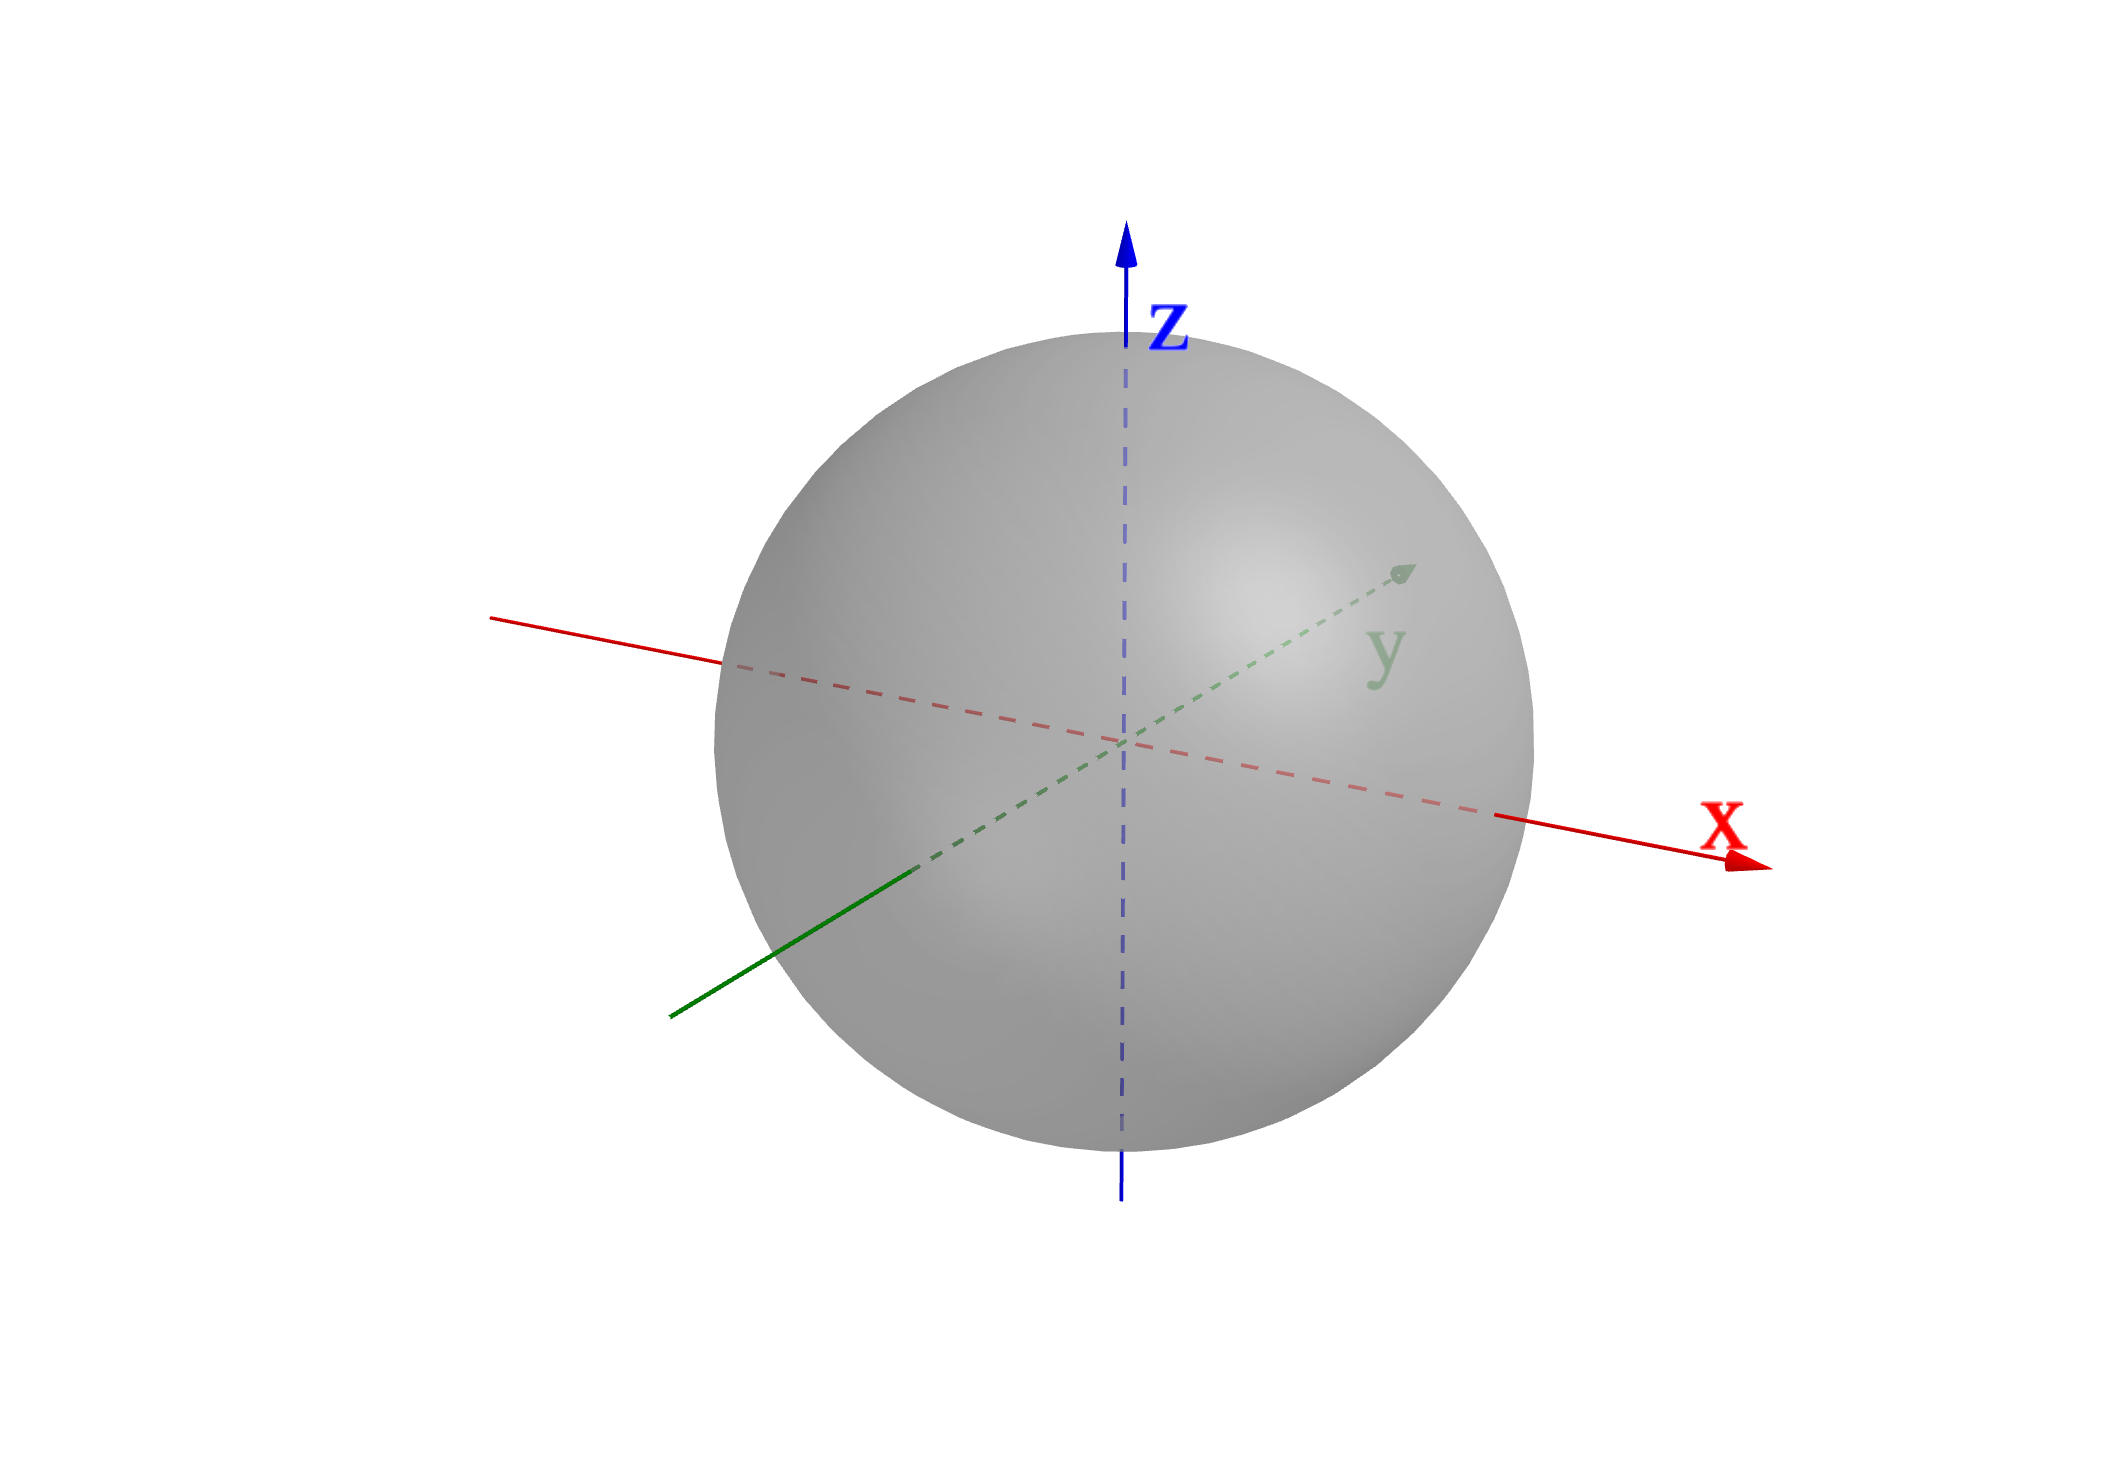
\includegraphics[width=0.5\textwidth]{Plots/sphere.png} \end{center}

\begin{definition}[Ellipsoid]\index{Ellipsoid}
    The 3D \term{ellipsoid} (with center) at the origin is given by $$\left(\frac{x}{a}\right)^2 + \left(\frac{y}{b}\right)^2 + \left(\frac{z}{c}\right)^2 = 1$$

    $(a, 0, 0)$, $(0, b, 0)$, $(0, 0, c)$ are the 3 points on the ellipsoid, similar to the ellipse.

    When $a = b = c$, an ellipsoid becomes a \term{sphere}, with $a = b = c = R$ as the radius.
\end{definition}

\begin{center} 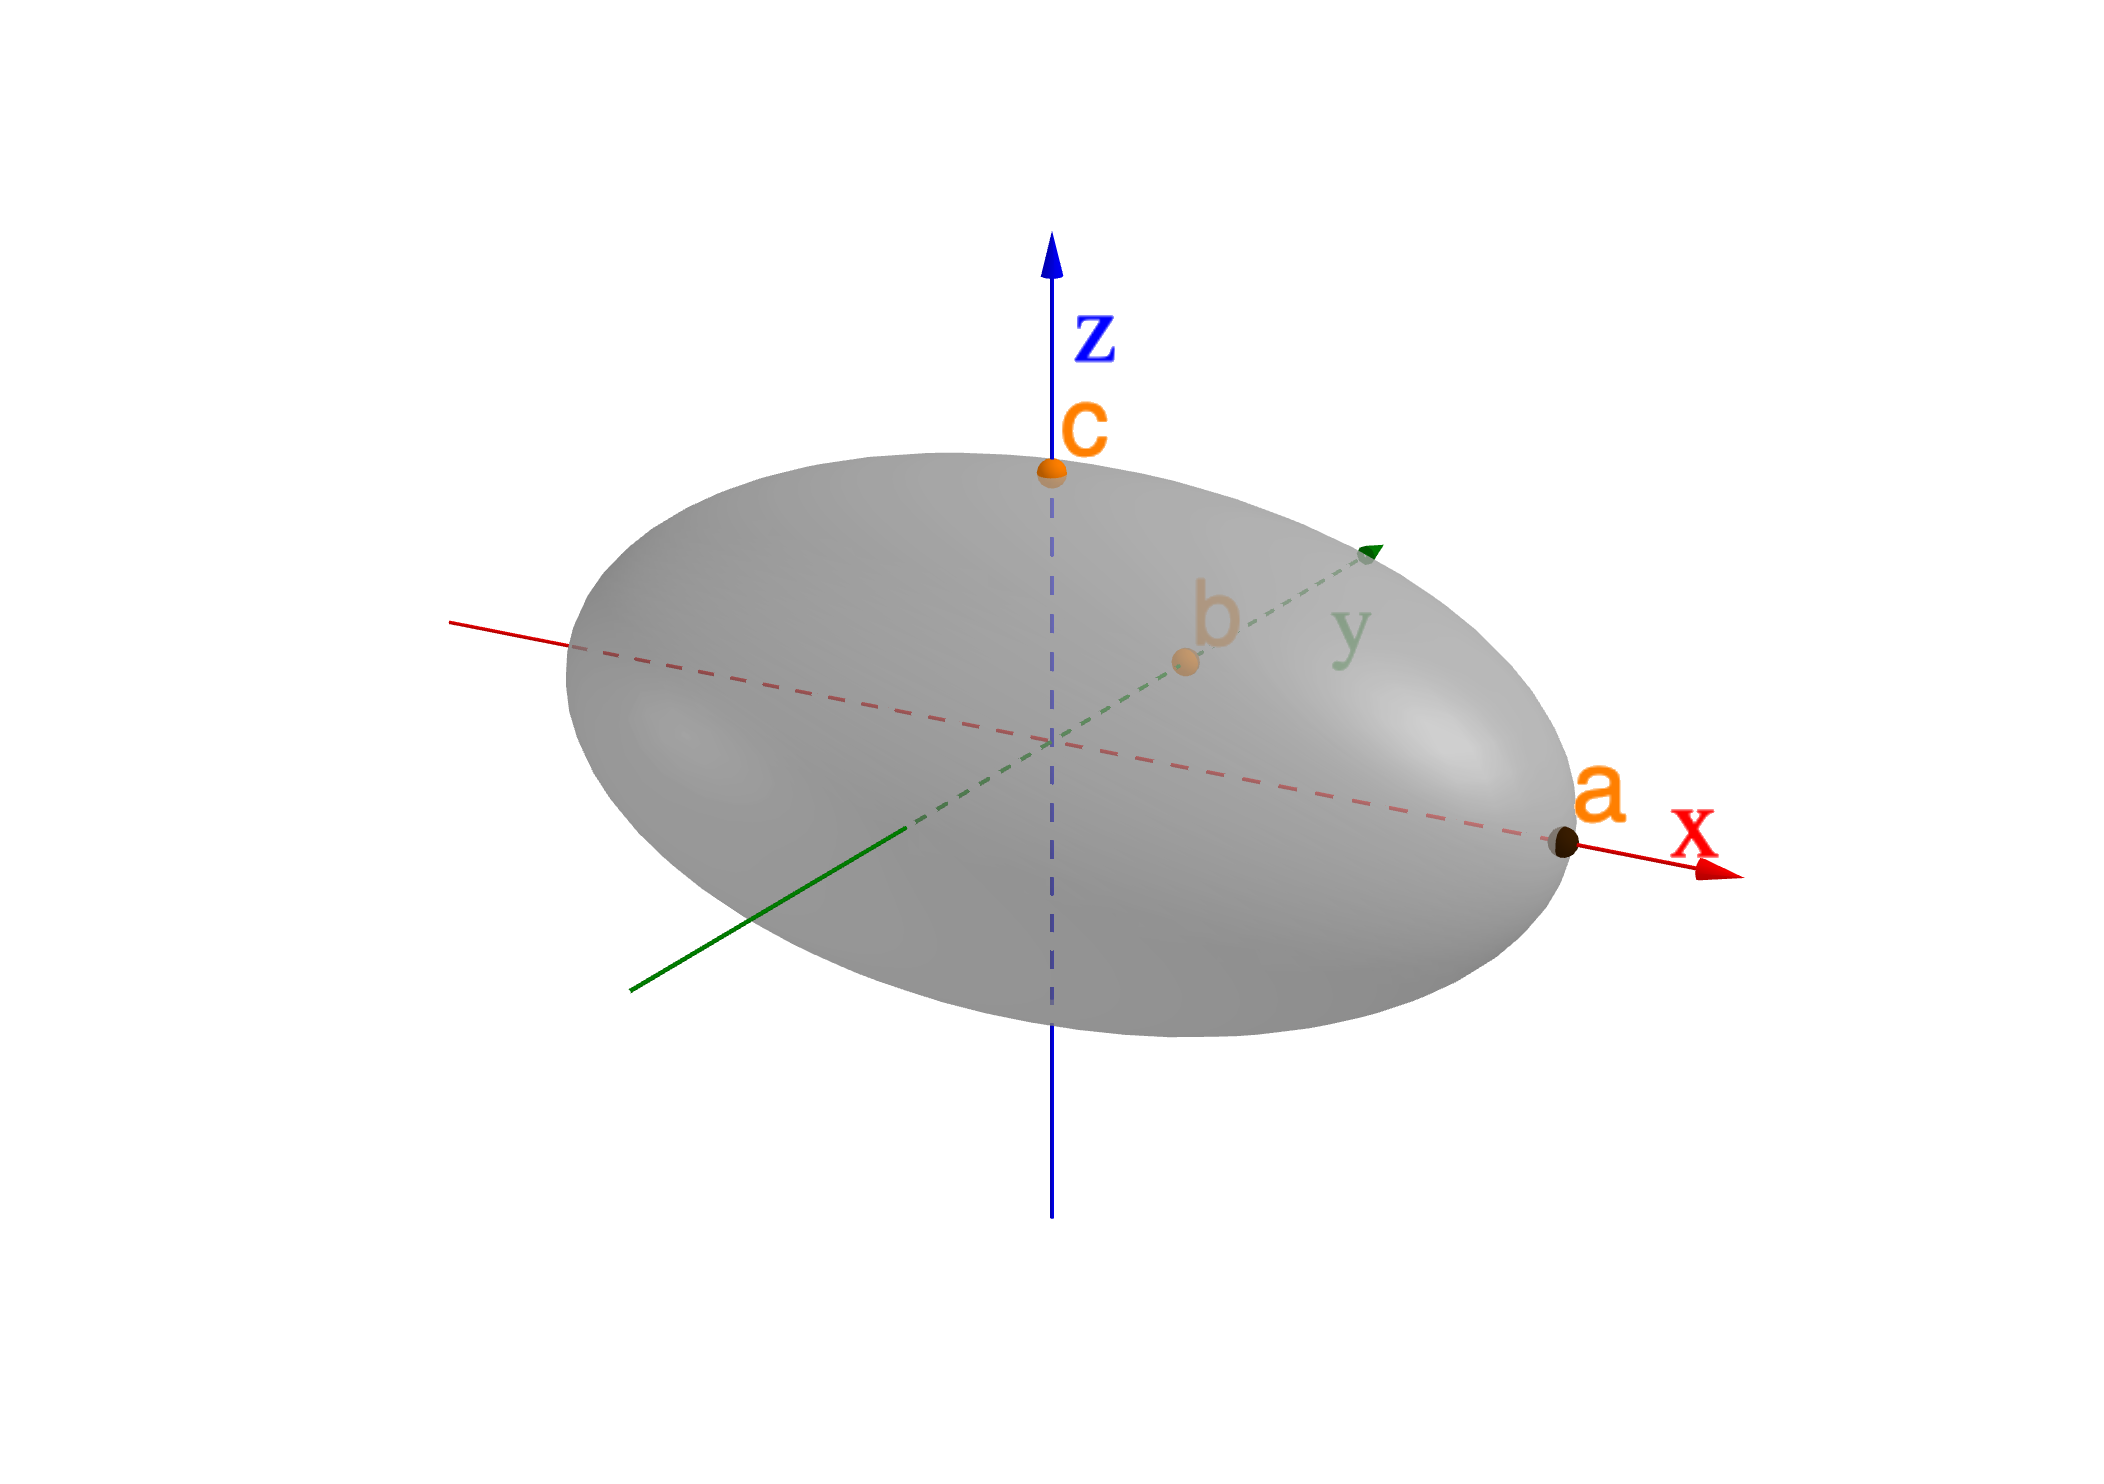
\includegraphics[width=0.5\textwidth]{Plots/ellipsoid.png} \end{center}

\subsubsection*{Surfaces Attained Through Rotation: $r^2 = x^2 + y^2$}

When the variables $x$ and $y$ appear together as $x^2 + y^2$, this signals that the surface is attained through rotation. Set a new variable $r$, with $r^2 = x^2 + y^2$. We graph the equation involving $z$ and $r$ in the $rz$-plane, with $r > 0$ only. We then revolve the curve around the $z$-axis to attain the surface in 3D: the $r$-axis stands for both $x$-axis and $y$-axis.

\begin{exercise}
    Sketch the following curves.

    \begin{minipage}[t]{0.45\linewidth} \setstretch{2.25}
        \begin{enumerate}
            \item $x = 2y^2$
            \item $\frac{x^2}{2} + \frac{y^2}{9} = 1$
            \item $x^2 + 2y^2 = 4$
        \end{enumerate}
    \end{minipage}
    \begin{minipage}[t]{0.45\linewidth} \setstretch{2.25}
        \begin{enumerate} \setcounter{enumi}{3}
            \item $x^2 + 3y^2 + 2x - 12y + 10 = 0$
            \item $y^2 - x^2 = 1$
            \item $\frac{(x - 2)^2}{4} - \frac{(y + 2)^2}{9} = 1$
        \end{enumerate}
    \end{minipage}
\end{exercise}

\begin{exercise}
    Sketch the following surfaces.

    \begin{minipage}[t]{0.45\linewidth} \setstretch{2.25}
        \begin{enumerate}
            \item $x^2 + y^2 = 1$

            \item $z = x^2 + y^2$

            \item $z^2 = x^2 + y^2$
        \end{enumerate}
    \end{minipage}
    \begin{minipage}[t]{0.45\linewidth} \setstretch{2.25}
        \begin{enumerate} \setcounter{enumi}{3}
            \item $x^2 + y^2 + \frac{z^2}{4} = 1$
            \item $z = \left( \sqrt{x^2 + y^2} - 1 \right)^2$
            \item $x^2 + y^2 + z^2 = 2z$
        \end{enumerate}
    \end{minipage}
\end{exercise}

\chapterimage{c2.png}

\chapter{Vectors and the Geometry of Space}

\section{Vector and Matrix}

A point in 2D needs 2 coordinates. It is typically written as, for example: $$\vec{a} = 1 \quad\text{or}\quad \vec{a} = \begin{bmatrix} 1 \\ 2 \end{bmatrix}$$ This is the point $x = 1$ and $y = 2$ on the 2D $xy$-plane.

A point in 3D needs 3 coordinates. It is typically written as, for example: $$\vec{b} = (0, 2, 1) \quad\text{or}\quad \vec{b} = \begin{bmatrix} 0 \\ 2 \\ 1 \end{bmatrix}$$ This is the point $x = 0$, $y = 2$, and $z = 1$ in 3D space.

The point can also be interpreted as a \term{vector}\index{Vector}, written in the same way. We can also think of a vector as an \itblue{arrow} from the origin to the point.

Typically, it doesn't matter if we write the vector horizontally or vertically.

\begin{definition}[Matrix]\index{Matrix}
    A \term{matrix} is a block of numbers written in a rectangle (or square) in a specific order.
\end{definition}

For example, A is a $2 \times 3$ (2 by 3) matrix, with 2 rows and 3 columns: $$A = \begin{bmatrix} a & b & c \\ d & e & f \end{bmatrix}$$

We may think of vectors as $1 \times n$ or $n \times 1$ matrix (for $n = 2$ or $3$). We can add matrices, and multiply matrices by a scalar (number).

{~~~}

\begin{itemize}
    \item $\begin{bmatrix} a & b \\ c & d \end{bmatrix} + \begin{bmatrix} e & f \\ g & h \end{bmatrix} = \begin{bmatrix} a + e & b + f \\ c + g & d + h \end{bmatrix}$
    \item $r\begin{bmatrix} a & b \\ c & d \end{bmatrix} = \begin{bmatrix} ra & rb & rc & rd \end{bmatrix}$
\end{itemize}

{~~~}

Standard arithmetic rules apply. For matrices $A$, $B$, and scalar $c$:

\begin{itemize}
    \item $A + B = B + A$
    \item $cA = Ac$
    \item $c(A + B) = cA + cB$
\end{itemize}

\section{Determinant}\index{Determinant}

The determinant of a \bred{square} matrix is a number.

Starting at the first row, first position, write down this value, and remove this row and this column from the original matrix. Multiply this value by the determinant of the remaining matrix.

$$\det \begin{bNiceMatrix} a & b & c \\ d & e & f \\ g & h & i \CodeAfter \tikz \draw (1-1) circle (1.8mm); \end{bNiceMatrix} = a \cdot \det \begin{bmatrix} e & f \\ h & i \end{bmatrix} \dots$$

Now, move right, write down this value, and remove this row and this column from the original matrix. Multiply this value to the determinant of the remaining matrix with a \bred{minus sign}.

$$\det \begin{bNiceMatrix} a & b & c \\ d & e & f \\ g & h & i \CodeAfter \tikz \draw (1-2) circle (1.8mm); \end{bNiceMatrix} = a \cdot \det \begin{bmatrix} e & f \\ h & i \end{bmatrix} {\color{red}-}~ b \cdot \det \begin{bmatrix} d & f \\ g & i \end{bmatrix}$$

Now, move right again and repeat until we have reached the last column. The positive and negative signs need to \bred{alternate}.

$$\det \begin{bNiceMatrix} a & b & c \\ d & e & f \\ g & h & i \CodeAfter \tikz \draw (1-3) circle (1.8mm); \end{bNiceMatrix} = a \cdot \det \begin{bmatrix} e & f \\ h & i \end{bmatrix} - b \cdot \det \begin{bmatrix} d & f \\ g & i \end{bmatrix} {\color{red}+}~ c \cdot \begin{bmatrix} d & e \\ g & h \end{bmatrix}$$

Each time we apply the algorithm, we end up with several new determinants to calculate, but with matrices of \itblue{smaller sizes}.

$$\det \begin{bmatrix} a & b \\ c & d \end{bmatrix} = ad = bc$$

Determinant does not behave well with addition and scalar multiplication:
$$\det(A + B) \neq \det(A) + \det(B) \qquad \det(cA) \neq c \cdot \det(A)$$

\begin{exercise}
    Find the determinant.

    {~~~}

    \begin{enumerate}
        \item $\begin{bmatrix} 3 & -1 \\ 2 & 5 \end{bmatrix}$

        {~~~}

        \item $\begin{bmatrix} 3 & 3 & -3 \\ -3 & -5 & 2 \\ -4 & 4 & -6 \end{bmatrix}$

        {~~~}

        \item $\begin{bmatrix} 3 & 1 & 0 \\ 1 & 3 & 4 \\ 0 & 0 & 4 \end{bmatrix}$
    \end{enumerate}
\end{exercise}

\section{Dot product}

2 vectors can form a \term{dot product}\index{Dot Product}, and the result is a scalar (number).

$$\vec{x} \cdot \vec{y} = \begin{bmatrix} x_1 \\ x_2 \\ \vdots \end{bmatrix} \cdot \begin{bmatrix} y_1 \\ y_2 \\ \vdots \end{bmatrix} = x_1y_1 + x_2y_2 + \cdots$$

Note that this dot product is different from scalar multiplication, as we are multiplying 2 vectors together, not a scalar with a vector.

The \term{length} (absolute value, or \term{norm})\index{length (of a Vector)}\index{Absolute Value (of a Vector)}\index{Norm} of a vector using the Pythagoras Theorem: $$| \vec{x} | = \sqrt{\vec{x} \cdot \vec{x}} = \sqrt{(x_1)^2 + (x_2)^2 + \cdots}$$

Similarly, define the distance between two points using pythagoras Theorem: $$d(\vec{x}, \vec{y}) = | \vec{x} - \vec{y} | = \sqrt{(y_1 - x_1)^2 + (y_2 - x_2)^2 + \cdots}$$

Going from a point a to point c, is always shorter than going to some other point b first and then back to c. This is called the \term{Triangle Inequality}\index{Triangle Inequality}: $$d(\vec{a},\vec{c}) \le d(\vec{a},\vec{b}) + d(\vec{b},\vec{c})$$ $$| \vec{x} + \vec{y} | \le | \vec{x} | + | \vec{y} |$$

Let $\theta$ be the angle between $\vec{x}$ and $\vec{y}$, the dot product is also given by $$\vec{x} \cdot \vec{y} = | \vec{x} | | \vec{y} | \cos \theta$$

Thus, 2 vectors are \term{orthogonal}\index{Orthogonal} (perpendicular\index{Perpendicular}) if the dot product is zero.

The dot product have the usual properties of multiplication:

\begin{itemize}
    \item $\vec{a} \cdot \vec{b} = \vec{b} \cdot \vec{a}$
    \item $\vec{a} \cdot (\vec{b} + \vec{c}) = \vec{a} \cdot \vec{b} + \vec{a} \cdot \vec{c}$
    \item $c(\vec{a} \cdot \vec{b}) = (c\vec{a}) \cdot \vec{b} = a \cdot (c\vec{b})$
\end{itemize}

Note that since the dot product needs two vectors and produce a number, a quantity such as $\vec{a} \cdot \vec{b} \cdot \vec{c}$ is not well defined.

\begin{exercise}
    Find the length of the vectors. Find $\vec{a} \cdot \vec{b}$ and the angle between them.

    {~~~}

    \begin{enumerate}
        \item $\vec{a} = (4, 3)$, $\vec{b} = (2, -1)$
        \item $\vec{a} = (4, 0, 2)$, $\vec{b} = (2, -1, 0)$
    \end{enumerate}
\end{exercise}

\section{Cross product}

2 vectors (in 3D) can form a \term{cross product}\index{Cross Product}, and the result is a \itblue{vector} (in 3D).

Let $\vec{x} = (x_1, x_2, x_3)$, $\vec{y} = (y_1, y_2, y_3)$ in 3D.

We typically write the cross product using determinant:

$$\vec{x} \times \vec{y} = \det \begin{bmatrix} i & i & k \\ x_1 & x_2 & x_3 \\ y_1 & y_2 & y_3 \end{bmatrix}$$ $$\vec{x} \times \vec{y} = i(x_2y_3 - x_3y_2) - j(x_1y_3 - x_3y_1) + k(x_1y_2 - x_2y_1)$$ $$\vec{x} \times \vec{y} = (x_2y_3 - x_3y_2, x_1y_3 - x_3y_1, x_1y_2 - x_2y_1)$$

The notations $i = (1, 0, 0)$, $j = (0, 1, 0)$, $k = (0, 0, 1)$ are very easy to use, where the quantity attached to $i$ is the first component of the vector, and the quantity attached to $j$ would be the second, and $k$ would be the third.

The vector produced by the cross product, $\vec{x} \times \vec{y}$, would be orthogonal to both vectors $\vec{x}$ and $\vec{y}$. Notice that in most cases, there would be 2 such vectors with this property. They are exactly $$\vec{x} \times \vec{y} \qquad\text{and}\qquad -\vec{x} \times \vec{y}$$

In fact, we have $$\vec{x} \times \vec{y} = - \vec{y} \times \vec{x}$$

Notice that the order of a dot product does not matter, but the order of cross product matters up to a negative sign.

The other usual properties of multiplication hold:

\begin{itemize}
    \item $(a\vec{a} \times \vec{b}) = c(\vec{a} \times \vec{b}) = a \times (c\vec{b})$
    \item $\vec{a} \times (\vec{b} + \vec{c}) = \vec{a} \times \vec{b} + \vec{a} \times \vec{c}$
\end{itemize}

Similar to the dot product, we can also relate the angle between the 2 vectors, $$| \vec{x} \times \vec{y} | = | \vec{x} | | \vec{y} | \sin \theta$$

Note that since $\vec{x} \times \vec{y}$ is a vector, we need to take its absolute value. So 2 vectors are \itblue{parallel} if the cross product is zero.

\begin{exercise}
    Let $\vec{x} = (3, -2, 1)$, $\vec{y} = (1, -1, 1)$. Find $\vec{x} \times \vec{y}$.
\end{exercise}

\section{Lines and Planes}

For a \term{line}\index{Line} to be defined, we need a direction $\vec{v}$ and a point on the line $\vec{r}_0$. $$\begin{bmatrix} x \\ y \\ z \end{bmatrix} := \vec{r} = t\vec{v} + \vec{r}_0$$

The vector $\vec{r}$ and the value $t$ do not need to be determined \footnote{$\vec{v}$ and $\vec{r}_0$ are not unique, and any correct pair would give the right equation. }.

For a \term{plane}\index{Plane} to be defined, we need a \bred{normal vector} $\vec{n} = (a, b, c)$ and a point on the plane $\vec{r}_0$. $$\vec{n} \cdot \vec{r} = \vec{n} \cdot \vec{r}_0$$ $$ax + by + cz = \vec{n} \cdot \vec{r}_0$$ where $\vec{r}$ is the same as above and does not need to be determined. The \term{normal vector}\index{Normal Vector (of a Plane)} $\vec{n}$ is orthogonal to the plane \footnote{Similar to lines, $\vec{v}$ and $\vec{r}_0$ are not unique. }.

\subsubsection*{Plane Defined by 3 Points}

Consider 3 points $\vec{u}$, $\vec{v}$, and $\vec{w}$. We can connect any 2 pairs of points together to create 2 direction vectors which are inside the plane. For example, we may take $\vec{x} = \vec{u} - \vec{v}$, and$ \vec{y} = \vec{w} - \vec{v}$. From there we can form the cross product to attain a vector that is orthogonal to both vectors inside the plane, so the cross product would be the normal vector, which is orthogonal to the plane.

\begin{exercise}
    Find the equation of the line or plane.

    {~~~}

    \begin{enumerate}
        \item The line through $(-8, 0, 4)$ and $(3, -2, 4)$.
        \item The plane through the origin and perpendicular to the vector $(1, 5, 2)$.
        \item The plane through $(2, 4, 6)$ parallel to the plane $x + y - z = 5$.
        \item The plane through $(0, 1, 1)$, $(1, 0, 1)$, and $(1, 1, 0)$.
        \item The plane equidistant from point $(3, 1, 5)$ and $(-2, 0, 0)$.
    \end{enumerate}
\end{exercise}

\chapterimage{c3.png}

\chapter{Partial Derivatives}

\section{Multivariable Function}

In first year, we study 1D functions: \term{functions of one variable}\index{Function of One Variable}, as $f(x)$. This can be plotted in 2D plane, with $y = f(x)$. Now, we can study functions of multiple variables.

\begin{definition}[2D Function]\index{2D Function}
    A \term{2D function}, $f(x, y)$, has 2 inputs being $x$, $y$, and 1 output.
\end{definition}

Sometimes, we can label the output as $z = f(x, y)$.

We can plot this 2D function in 3D space, where the height $z$ above the point $(x, y)$ on the $xy$-plane is equal to $f(x, y)$.

This would give a graph, which is a surface.

Alternatively, $z = f(x, y)$ can be thought of as an equation which involves $x$, $y$, and $z$, which would also give a surface in 3D space.

However, similar to 1D functions, given an equation involving $x$, $y$, and $z$, it is not always possible to isolate $z$ into $z = f(x, y)$.

Examples of 2D functions include: $$f(x, y) = x^2 + 2y \qquad f(x, y) = xe^{xy} \qquad f(x, y) = \sin(xy^2)$$

\begin{definition}[3D Function]\index{3D Function}
    A \term{3D function}, $f(x, y, z)$, has 3 inputs being $x$, $y$, and $z$, and 1 output.
\end{definition}

It is possible to label the output as $w = f(x, y, z)$, but this is typically not useful as this introduces a 4th variable. The ``plot'' of this function would be in 4D space, which does not exist.

Examples of 3D functions include: $$f(x, y, z = x^2 + 2z - 1) \qquad f(x, y, z) = ye^{xz}$$

\begin{definition}[Level Set]\index{Level Set}
    The \term{level set} of $f$ at $k$ is given by setting $f$ to be equal to the constant $k$. This will reduce the dimension of $f$ by 1.
\end{definition}

\begin{exercise}
    $\text{ }$

    \begin{itemize}
        \item Draw the level set of $f(x, y) = 4x^2 + y^2 + 1$ for $k = 2$ and $k = 5$.
        \item Draw the level set of $f(x, y, z) = x^2 + y^2 - z$ for $k = 0$ and $k = 2$.
    \end{itemize}
\end{exercise}

\section{Limits and Continuity}

$f(x, y)$ is continuous at the 2D point $\vec{a}$ if $$\lim_{(x, y) \to \vec{a}} f(x, y) = f(\vec{a})$$

Every standard function we know are continuous in their domains. Any function transformations (such as $+$, $-$, $\times$, $/$, composition) of continuous functions, are also continuous (except division by $0$).

As most functions are continuous, most limits can be obtained by putting $(x, y) = \vec{a}$ in the formula of $f(x,y)$.

Different from 1D functions, computing limits in 2D is much more difficult. Most limit evaluation techniques from 1D functions does not work for 2D functions. In particular, there is no L'Hôpital's rule Rule for 2D functions.

Fortunately, since most functions are continuous except when dividing by $0$, we typically only need to focus on the point where the function is dividing by $0$ (and state the function is continuous everywhere else).

It turns out that it is much easier to show a limit does not exist.

\subsubsection{Test for limit that does not exist in $\mathbb{R}^2$}

Given $f(x, y)$, compute the limit as $(x, y)$ approaches $\vec{a} = (0, 0)$.

\begin{enumerate}
    \item Replace $y$ with a easy curve $y = g(x)$, passing through $\vec{a} = (0, 0)$, (such as $y = 0$, $y = x$, $y = x^2$), then let $x$ approach $0$ to attain a (1D) limit.
    \item Replace $x$ with a easy curve $x = h(y)$, passing through $\vec{a} = (0, 0)$, (such as $x = 0$, $x = y^2$), then let $y$ approach $0$ to attain a (1D) limit.
    \item Try with several different $g(x)$ and $h(y)$ to attain many (1D) limits.
    \item If you find 2 \bred{different} (1D) limits generated by 2 different curves, then the (2D) limit of $(x, y)$ approaches $\vec{a} = (0, 0)$ of $f(x, y)$ does not exist.
\end{enumerate}

Note that if all the 1D limits are the same, that is \bred{not} enough for you to conclude the 2D limit exists. To show the limit exists, we typically must use \itblue{Squeeze Theorem}.

Since most limit evaluation techniques does not work for 2D functions, it is a very fortunate fact that Squeeze Theorem does work for 2D functions. The formulation is almost the same as the 1D version.

\begin{theorem}[Squeeze Theorem]\index{Squeeze Theorem}
    {~~~}

    To attain $\lim_{(x, y) \to \vec{a}} f(x, y)$, we can try to find $g(x, y)$ and $h(x, y)$ such that

    \begin{enumerate}
        \item $g(x, y) \le f(x, y) \le h(x, y)$ near the point $\vec{a}$
        \item $\lim_{(x, y) \to \vec{a}} g(x, y) = L = \lim_{(x, y) \to \vec{a}} h(x,y)$
    \end{enumerate}

    Then we conclude $\lim_{(x, y) \to \vec{a}} f(x, y) = L$.
\end{theorem}

\subsubsection{Use Squeeze Theorem to show limit exist}

In practice, we typically want to show $\lim_{(x, y) \to \vec{a}} f(x, y) = 0$.

Start at $| f(x, y) |$, create a \itblue{chain of inequalities}, and simplify $| f(x, y) |$ to attain $| g(x, y) |$, which has limit $0$ as $(x, y)$ approaches $\vec{a}$: $$|f(x, y)| \le \cdots \le | g(x, y) | \to 0 \quad\text{i.e.}\quad \lim_{(x, y) \to \vec{a}} | g(x, y) | = 0$$ Then we conclude $\lim_{(x, y) \to \vec{a}} f(x, y) = 0$.

The typical strategy in constructing the above inequality is to remove positive quantities from the denominator of $f(x, y)$.

\begin{exercise}
    $$f(x, y) = \frac{x^2y}{x^4 + y^2} \quad\text{and}\quad f(0, 0) = 0$$

    Show the limit at $(x, y) = (0, 0)$ does not exist.
\end{exercise}

\begin{exercise}
    $$f(x, y) = \frac{xy}{\sqrt{x^4 + y^2}} \quad\text{and}\quad f(0, 0) = 0$$

    Show the function \textbf{continuous} at $(0, 0)$.
\end{exercise}

\begin{exercise}
    Find $\lim_{(x, y) \to (0, 0)} \frac{x^2 \sin^2{y}}{2x^4 + y^2}$
\end{exercise}

\section{Derivative}

Consider multivariable function $f(x, y)$ or $f(x, y, z)$.

Define the \term{derivative}\index{Derivative} to be:
$$\begin{aligned}[t]
    & \text{For } f(x, y)    &  & \Delta f = \left( \frac{\partial f}{\partial x}, \frac{\partial f}{\partial y} \right)                                \\
    & \text{For } f(x, y, z) &  & \Delta f = \left( \frac{\partial f}{\partial x}, \frac{\partial f}{\partial y}, \frac{\partial f}{\partial z} \right)
\end{aligned}$$
where $\Delta f$ is called \term{`del' $f$}\index{`del'}, or \term{gradient}\index{Gradient} of $f$.

We can interpret $\Delta f$ as a vector, even though $f(x, y)$ or $f(x, y, z)$ is a scalar.

The quantities in $\Delta f$ such as $\frac{\partial f}{\partial x}$ are called \term{partial derivatives}\index{Partial Derivative}. When taking partial derivatives with respect to a variable, we regard \bred{all other variables} as \itblue{constants} and take the derivative as usual. Sometimes, we use the notations $$\frac{\partial f}{\partial x} = f_x \qquad \frac{\partial f}{\partial y} = f_y \qquad \frac{\partial f}{\partial z} = f_z$$

\begin{example}
    Let $f(x, y) = x^2 y^3 + x$. 

    To take the partial derivative with respect to $x$, $\frac{\partial f}{\partial x}$, we view $y$ as constant. 
    $$\frac{\partial f}{\partial x} = 2xy^3 + 1$$

    To take the partial derivative with respect to $y$, $\frac{\partial f}{\partial y}$, we view $x$ as constant. 
    $$\frac{\partial f}{\partial y} = 3x^2y^2$$
\end{example}

\begin{example}
    Let $f(x, y, z) = x^2z + yz^2$. 

    To take the partial derivative with respect to $x$, $\frac{\partial f}{\partial x}$, we view \bred{both} $y$ and $z$ as constants. Similarly, for other partial derivatives, 
    $$\frac{\partial f}{\partial x} = 2xz \qquad \frac{\partial f}{\partial y} = z^2 \qquad \frac{\partial f}{\partial z} = x^2 + 2yz$$
\end{example}

\begin{exercise}
    Computer $\Delta f$. 

    \begin{minipage}[t]{0.45\linewidth} \setstretch{2}
        \begin{enumerate}
            \item $f(x, y) = (x^2 - 1)(y + 1)$
            \item $f(x, y) = (xy - 2)^2$
            \item $f(x, y) = \frac{2}{x + 3y}$
        \end{enumerate}
    \end{minipage}   
    \begin{minipage}[t]{0.45\linewidth} \setstretch{2}
        \begin{enumerate}
            \setcounter{enumi}{3}
            \item $f(x, y) = x^{x + 4y}$
            \item $f(x, y, z) = x^2 + 2z - 1$
            \item $f(x, y, z) = ye^{xz}$
        \end{enumerate}
    \end{minipage}   
\end{exercise}

\section{Directional Derivative}

Remember one dimensional derivatives in first year?
$$f'(a) = \lim_{h \to 0} \frac{f(a + h) - f(a)}{h}$$ where $f$ is defined on the real line.

We start at the point $x = a$, and we ask, if we move just a tiny bit away from $x = a$, how much does the function change?

We generalize this idea of moving a tiny bit away in higher dimensions. In the real line, we can move only left or right. In 2D, we can move in any direction we like (on the plane).

We can describe the direction of movement by a \term{unit vector}, similar to the direction vector of the equation of a line. The \term{directional derivative}\index{Directional Derivative} toward the direction $\vec{u}$ at the point $\vec{a}$ \footnote{This is a 1D limit, as $h$ is a number (the length of the movement). }: $$D_{\vec{u}} f(\vec{a}) = \lim_{h \to 0} \frac{f(\vec{a} + h\vec{u}) - f(\vec{a})}{h}$$ 

This is also the \term{rate of change}\index{Rate of Change} of the function in the direction $\vec{u}$ at the point $\vec{a}$. 

Given a vector $\vec{v}$, we can turn it into a \term{unit vector} $\vec{u} = \frac{\vec{v}}{| \vec{v} |}$. 

\begin{definition}[Unit Vector]\index{Unit Vector}
    A \term{unit vector} is a vector whose length (norm) is exactly $1$. 
\end{definition}

{~~~}

Some useful facts:

\begin{enumerate}
    \item Partial derivatives are directional derivatives with $\vec{u}$ being in a \term{coordinate direction}. For example, for $f(x,y)$, 

    \begin{itemize}
        \item $\frac{\partial f}{\partial x} = D_{\vec{u}} f$ with $\vec{u} = (1, 0)$;
        \item $\frac{\partial f}{\partial y} = D_{\vec{u}} f$ with $\vec{u} = (0, 1)$;
    \end{itemize}

    {~~~}

    \item If $f$ is \bred{differentiable}, then all directional derivative exist and $$D_{\vec{u}} f = \Delta f \dot \vec{u}$$ where $\vec{u}$ is a \bred{unit vector}. 
    
    This formula gives an easy way to calculate directional derivative.

    {~~~}

    \item We can interpret $\Delta f(\vec{a})$ as a vector. 
    
    If we evaluate $\Delta f$ at a point $\vec{a}$, and if we interpret the vector $\Delta f(\vec{a})$ as a direction, then the directional derivative in the direction of $\Delta f(\vec{a})$ at the point $\vec{a}$ is the largest, and the value of this maximum directional derivative is equal to $| \Delta f(\vec{a}) |$. 

    {~~~}

    \item Recall equation of plane: $\vec{n} \cdot \vec{r} = \vec{n} \cdot \vec{r}_0$
    
    For $f(x, y, z) = k$ for some constant $k$, gives a \term{level set} surface. Define the \term{tangent plane} at some fixed point $\vec{r}_0 = (x_0, y_0, z_0)$ by the \bred{normal vector} $\vec{n} = \Delta f(x_0, y_0, z_0)$.
\end{enumerate}

\begin{exercise}
    $f(x, y, z) = e^{2x}y + y^2 + 4$. At the point $(0, 0)$, find the directional derivative along the direction given by $\vec{u} = (1, 3)$ (first turn $\vec{v}$ into a unit vector). 
\end{exercise}

\begin{exercise}
    $f(x, y, z) = x^2y + z$. At the point $(2, 2, 1)$, find the maximum rate of change, and the direction with the maximum (the direction with maximum rate of change is $\Delta f$, and the value of this maximum rate of change is $| \Delta f |$). 
\end{exercise}

\begin{exercise}
    Define $f(x, y, z) = xy^2e^z$. Let $f(x, y, z) = e$. 

    At the point $(1, 1, 1)$, find the equation of the tangent plane.
\end{exercise}

\begin{exercise}
    Find all directional derivatives at $(0, 0)$ (including the partials), if they exist. Is the function \textbf{continuous} at $(0, 0)$?
    \begin{enumerate}[label=\alph*)]
        \item 
        $f(x, y) = \begin{cases}
            \frac{xy}{x^2 + y^2} & (x, y) \neq (0, 0) \\
            0                    & (x, y) = (0, 0)
        \end{cases}$

        \item $f(x, y) = \sqrt{|xy|}$
    \end{enumerate}

    {~~~}

    \textbf{Strategy:}

    When the function has division by $0$, or some other problems at the origin (such as absolute value or square root), we must use the definition of directional derivative, because $f$ \bred{may not be differentiable} at $(0, 0)$ so the formula $\Delta f \cdot \vec{u}$ does not work. Set $\vec{a} = (0, 0)$ and $\vec{u} = (a, b)$ where $a^2 + b^2 = 1$. 
\end{exercise}

\section{Differentiation}

\begin{definition}[Differentiable]\index{Differentiable}
    $f$ is \term{differentiable} if the gradient vector $\Delta f(\vec{a})$ satisfies $$\lim_{\vec{h} \to \vec{0}} = \frac{f(\vec{a} + \vec{h}) - f(\vec{a}) - \Delta f(\vec{a}) \cdot \vec{h}}{| \vec{h} |} = 0$$
\end{definition}

Note that this is a \itblue{2D limit}. This limit is typically used when $\vec{a} = (0, 0)$, so we may set $\vec{h} = (x, y)$ and show the limit is zero using Squeeze Theorem.

{~~~}

Some useful facts:

\begin{enumerate}
    \item If $f$ is $C^1$ at $\vec{a}$ \footnote{This means all partial derivatives exist near $\vec{a}$ and at $\vec{a}$, and the partial derivatives are \bred{continuous} (as functions) at $\vec{a}$. }, then $f$ is differentiable at $\vec{a}$ ($\Delta f$ exists). 

    \item Being differentiable is a stronger condition than having directional derivative. If $f$ is differentiable, then all directional derivative is given by $D_{\vec{u}} f = \Delta f \cdot \vec{u}$. 

    \item If a function $f$ is differentiable at $\vec{a}$, then $f$ is continuous at $\vec{a}$.
\end{enumerate}

{~~~}

\begin{exercise}
    Define $$f(x, y) = \begin{cases}
        \frac{xy}{x^2 + y^2} & (x, y) \neq (0, 0) \\
        0                    & (x, y) = (0, 0)
    \end{cases}$$

    Show the directional derivatives exist at $(0, 0)$, but $f$ is \textbf{not differentiable} at $(0, 0)$.

    {~~~}

    \textbf{Strategy:}
    
    There are 2 ways to approach the problem.

    \begin{enumerate}
        \item If the function is \textbf{not continuous} at $(0, 0)$, then it is \textbf{not differentiable} at $(0, 0)$. So we may try to show it is not continuous at $(0, 0)$. However, some functions \textbf{are continuous} at $(0, 0)$, so we can attain no conclusion in such cases.

        \item Compute all the directional derivatives. If $f$ is differentiable, then every directional derivative should satisfy $D_{\vec{u}} = \Delta f \cdot \vec{u}$. 
        
        Check this equation for $\vec{u} = (1, 0)$, $\vec{u} = (0, 1)$, and $\vec{u} = \left( \frac{1}{\sqrt{2}}, \frac{1}{\sqrt{2}} \right)$ (easy unit vectors). 
    \end{enumerate}
\end{exercise}

\begin{exercise}
    Show whether the function is differentiable at $(0, 0)$.

    \begin{enumerate}[label=\alph*)]
        \item $f(x, y) = \begin{cases}
            \frac{x|y|}{\sqrt{x^2 + y^2}} & (x, y) \neq (0, 0) \\
            0                             & (x, y) = (0, 0)
        \end{cases}$

        \item $f(x, y) = \begin{cases}
            \frac{x^4 + y^4}{x^2 + y^2} & (x, y) \neq (0, 0) \\
            0                           & (x, y) = (0, 0)
        \end{cases}$
    \end{enumerate}
\end{exercise}

\section{Higher Order Derivative}

We may take (partial) derivatives on top of partial derivatives. 

In 2 dimensions, for $f(x, y)$, there are 4 ways of taking second derivatives. We put them into the \term{Hessian Matrix}\index{Hessian Matrix}: 
$$H = \begin{bmatrix}
    \frac{\partial^2 f}{\partial x^2} & \frac{\partial^2 f}{\partial xy}  \\
    \frac{\partial^2 f}{\partial yx}  & \frac{\partial^2 f}{\partial y^2}
\end{bmatrix} = \begin{bmatrix}
    \frac{\partial f}{\partial x}\left( \frac{\partial f}{\partial x} \right) & 
    \frac{\partial f}{\partial x}\left( \frac{\partial f}{\partial y} \right)   \\
    \frac{\partial f}{\partial y}\left( \frac{\partial f}{\partial x} \right) & 
    \frac{\partial f}{\partial y}\left( \frac{\partial f}{\partial y} \right)
\end{bmatrix} = \begin{bmatrix}
    f_{xx} & f{xy} \\ f{yx} & f{yy}
\end{bmatrix}$$

{~~~}

If $f$ is $C^2$ at $\vec{a}$ \footnote{This means all the 2nd order partial derivatives exist near $\vec{a}$ and at $\vec{a}$, and the 2nd order partial derivatives are continuous (as functions) at $\vec{a}$ (In practice, a function can fail to be continuous when there is division by zero). }, then \bred{mixed partial derivatives commute}:

The order of taking derivatives does not change the final answer: $f_{xy} = f_{yx} \to$ Taking derivative in $x$ then $y$ is the same as taking in $y$ then $x$.

In other words, if $f$ is $C^2$, then \bred{the Hessian Matrix is symmetric}.

{~~~}

We can also construct the Hessian for $f(x, y, z)$, which will be a $3 \times 3$ matrix. We can also construct higher order derivatives, such as 3rd order $f_{xyz}$ or $f_{xyy}$. In general, if $f$ is $C^k$, then mixed partial derivatives commute (up to order $k$).

\begin{exercise}
    Find the Hessian Matrix.

    \begin{minipage}[t]{0.45\linewidth} \setstretch{1.5}
        \begin{enumerate}
            \item $f(x, y) = 3x^2 + 4xy + 5y^2$
            \item $f(x, y) = \cos(x + 2y)$
            \item $f(x, y) = x^{2x + y}$
        \end{enumerate}
    \end{minipage}
    \begin{minipage}[t]{0.45\linewidth} \setstretch{1.5}
        \begin{enumerate} \setcounter{enumi}{3}
            \item $f(x, y) = e^{x^2 + y}$
            \item $f(x, y) = e^x \sin(y)$
            \item $f(x, y, z) = x^2y + xz + z^2$
        \end{enumerate}
    \end{minipage}
\end{exercise}

\begin{exercise}
    $$f(x, y) = \begin{cases}
        \frac{x^3y - xy^3}{x^2 + y^2} & (x, y) \neq (0, 0) \\
        0                             & (x, y) = (0, 0)
    \end{cases}$$

    Find $f_x$ and $f_y$ at $(x, y) = (0, 0)$ \textbf{and} $(x, y) \neq (0, 0)$. Then show $f_{xy} \neq f_{yx}$ at $(0, 0)$. i.e. Taking 2nd derivatives in different orders give different answers. 

    Is $f$ $C^2$ at $(0, 0)$ (and have we reacher a contradiction)?
\end{exercise}

%----------------------------------------------------------------------------------------
%	APPENDICES
%----------------------------------------------------------------------------------------

\part{Appendices}

\chapterimage{sol.png}

\chapter*{Solutions to Exercise Questions}
\addcontentsline{toc}{chapter}{\textcolor{ocre}{A Solutions to Exercise Questions}}
\setlength{\parindent}{0pt} % No indentation

\section*{Chapter 1}

\subsection*{Exercise 1.1}

\begin{enumerate}
    \item
    \begin{minipage}[t]{0.45\linewidth}
        $x = 2y^2$
    \end{minipage}
    \begin{minipage}[t]{0.45\linewidth}
        \begin{center}
            \begin{tikzpicture}[baseline=(current bounding box.west)]
                \draw[->] (-0.5, 0) -- (2.5, 0) node[right] {$x$};
                \draw[->] (0, -1.5) -- (0, 1.5) node[above] {$y$};

                \draw[thick,blue,domain=0:2] plot (\x, {sqrt(\x)});
                \draw[thick,blue,domain=0:2] plot (\x, {-sqrt(\x)});
            \end{tikzpicture}
        \end{center}
    \end{minipage}

    \item
    \begin{minipage}[t]{0.45\linewidth}
        $\begin{aligned}[t]
            \frac{x^2}{2} + \frac{y^2}{9}                                  & = 1 \\
            \left(\frac{x}{\sqrt{2}}\right)^2 + \left(\frac{y}{3}\right)^2 & = 1
        \end{aligned}$
    \end{minipage}
    \begin{minipage}[t]{0.45\linewidth}
        \begin{center}
            \begin{tikzpicture}[baseline=(current bounding box.west)]
                \draw[->] (-1.12, 0) -- (1.12, 0) node[right] {$x$};
                \draw[->] (0, -2) -- (0, 2) node[above] {$y$};

                \draw[thick,blue] (0, 0) ellipse (0.8cm and 1.68cm);

                \draw[thick,red] (0.8, 0.25) -- (0.8, 0) node[below,red] {$\sqrt{2}$};
                \draw[thick,red] (-0.8, 0.25) -- (-0.8, 0) node[below,red] {$-\sqrt{2}$};
                \draw[thick,red] (0.25, 1.68) -- (0, 1.68) node[left,red] {$3$};
                \draw[thick,red] (0.25, -1.68) -- (0, -1.68) node[left,red] {$-3$};
            \end{tikzpicture}
        \end{center}
    \end{minipage}

    \item
    \begin{minipage}[t]{0.45\linewidth}
        $\begin{aligned}[t]
            x^2 + 2y^2                                                     & = 4 \\
            \frac{x^2}{4} + \frac{2y^2}{4}                                 & = 1 \\
            \left(\frac{x}{2}\right)^2 + \left(\frac{y}{\sqrt{2}}\right)^2 & = 1
        \end{aligned}$
    \end{minipage}
    \begin{minipage}[t]{0.45\linewidth}
        \begin{center}
            \begin{tikzpicture}[baseline=(current bounding box.north west)]
                \draw[->] (-1.92, 0) -- (1.92, 0) node[right] {$x$};
                \draw[->] (0, -1.44) -- (0, 1.44) node[above] {$y$};

                \draw[thick,blue] (0, 0) ellipse (1.6cm and 1.12cm);

                \draw[thick,red] (1.6, 0.25) -- (1.6, 0) node[below,red] {$2$};
                \draw[thick,red] (-1.6, 0.25) -- (-1.6, 0) node[below,red] {$-2$};
                \draw[thick,red] (0.25, 1.12) -- (0, 1.12) node[left,red] {$\sqrt{2}$};
                \draw[thick,red] (0.25, -1.12) -- (0, -1.12) node[left,red] {$-\sqrt{2}$};
            \end{tikzpicture}
        \end{center}
    \end{minipage}

    \item
    \begin{minipage}[t]{0.45\linewidth}
        $\begin{aligned}[t]
            x^2 + 3y^2 + 2x - 12y + 10                                             & = 0 \\
            (x^2 + 2x + 1) + 3(y^2 - 4y + 4) - 3                                   & = 0 \\
            (x + 1)^2 + 3(y - 2)^2                                                 & = 3 \\
            \left(\frac{x + 1}{\sqrt{3}}\right)^2 + \left(\frac{y - 2}{1}\right)^2 & = 1
        \end{aligned}$

        Ellipse before the shift (in {\color{DarkGreen}green}): $$\left(\frac{x}{\sqrt{3}}\right)^2 + \left(\frac{y}{1}\right)^2 = 1$$

        Then, shift $1$ unit left and $2$ units up.
    \end{minipage}
    \begin{minipage}[t]{0.45\linewidth}
        \begin{center}
            \begin{tikzpicture}[baseline=(current bounding box.north)]
                \draw[->] (-3.2, 0) -- (2.2, 0) node[right] {$x$};
                \draw[->] (0, -1.2) -- (0, 3.7) node[above] {$y$};

                \draw[thick,DarkGreen] (0, 0) ellipse (1.7cm and 1cm);
                \draw[thick,blue] (-1, 2) ellipse (1.7cm and 1cm);

                \draw[thick,orange] (1.7, 0.25) -- (1.7, 0) node[below] {$\sqrt{3}$};
                \draw[thick,orange] (0.25, 1) -- (0, 1) node[left,red] {$1$};

                \draw[thick,red,dashed] (0.7, 2) -- (0.7, 0) node[below] {$\sqrt{3} - 1$};
                \draw[thick,red,dashed] (-2.7, 2) -- (-2.7, 0) node[below] {$-\sqrt{3} - 1$};

                \draw[thick,red,dashed] (-1, 2) -- (0, 2) node[left] {$2$};
                \draw[thick,red,dashed] (-1, 2) -- (-1, 0) node[below] {$-1$};

                \draw[thick,red,dashed] (-1, 3) -- (0, 3) node[left] {$3$};
                \draw[thick,red,dashed] (-1, 1) -- (0, 1);
            \end{tikzpicture}
        \end{center}
    \end{minipage}

    \item
    \begin{minipage}[t]{0.45\linewidth}
        $y^2 - x^2 = 1$

        {~~~}

        If $y = 0$, then $-x^2 = 1$, not possible.

        Thus, the graph must not cross the horizontal axis, and the hyperbola opens \bred{up and down}.

        {~~~}

        If $x = 0$, then $y^2 = 1$, $y = \pm 1$.
    \end{minipage}
    \begin{minipage}[t]{0.45\linewidth}
        \begin{center}
            \begin{tikzpicture}[baseline=(current bounding box.north)]
                \draw[->] (-2.2, 0) -- (2.2, 0) node[right] {$x$};
                \draw[->] (0, -2.2) -- (0, 2.2) node[above] {$y$};

                \clip(-2, -2) rectangle (2, 2);

                \draw[thick,blue,rotate around={90:(0,0)},domain=-0.99:0.99] plot ({( 1+(\x)^2)/(1-(\x)^2)}, {  2 *(\x)/(1-(\x)^2)});
                \draw[thick,blue,rotate around={90:(0,0)},domain=-0.99:0.99] plot ({(-1-(\x)^2)/(1-(\x)^2)}, {(-2)*(\x)/(1-(\x)^2)});

                \draw[red] (0.25,-1) -- (0,-1) node[left] {$-1$};
                \draw[red] (0.25,1) -- (0,1) node[left] {$1$};
            \end{tikzpicture}
        \end{center}
    \end{minipage}

    \item
    \begin{minipage}[t]{0.45\linewidth}
        $\begin{aligned}[t]
            \frac{(x-2)^2}{4} - \frac{(y+2)^2}{9}                       & = 1 \\
            \left(\frac{x-2}{2}\right)^2 - \left(\frac{y+2}{3}\right)^2 & = 1
        \end{aligned}$

        {~~~}

        Hyperbola before the shift (in {\color{DarkGreen}green}): $$\left(\frac{x}{2}\right)^2 - \left(\frac{y}{3}\right)^2 = 1$$

        If $x = 0$, then $-y^2 = 1$, not possible.

        Thus, the graph must not cross the vertical axis, and the hyperbola opens \bred{left and right}.

        If $y = 0$, then $\left(\frac{x}{2}\right)^2 = 1$, $x = \pm 2$.
    \end{minipage}
    \begin{minipage}[t]{0.45\linewidth}
        \begin{center}
            \begin{tikzpicture}[baseline=(current bounding box.north)]
                \draw[->] (-2.2, 0) -- (3.2, 0) node[right] {$x$};
                \draw[->] (0, -2.7) -- (0, 2.7) node[above] {$y$};

                \clip(-3, -2.5) rectangle (3, 2);

                \draw[thick,DarkGreen,domain=-0.99:0.99] plot ({( 1+(\x)^2)/(1-(\x)^2)}, {  2 *(\x)/(1-(\x)^2)});
                \draw[thick,DarkGreen,domain=-0.99:0.99] plot ({(-1-(\x)^2)/(1-(\x)^2)}, {(-2)*(\x)/(1-(\x)^2)});

                \draw[thick,blue,domain=-0.99:0.99] plot ({( 1+(\x)^2)/(1-(\x)^2) + 1}, {  2 *(\x)/(1-(\x)^2) - 1});
                \draw[thick,blue,domain=-0.99:0.99] plot ({(-1-(\x)^2)/(1-(\x)^2) + 1}, {(-2)*(\x)/(1-(\x)^2) - 1});

                \draw[thick,red,dashed] (2,-1) -- (0,-1) node[left] {$-2$};
                \draw[thick,red,dashed] (2,-1) -- (2,0) node[below] {$4$};
                \draw[thick,red,dashed] (1,0) -- (1,-1) node[below] {$(2,-2)$};

                \draw[orange] (-1,0.25) -- (-1,0) node[below] {$-2$};
                \draw[orange] (1,0.25) -- (1,0) node[below] {$2$};
            \end{tikzpicture}
        \end{center}
    \end{minipage}
\end{enumerate}

\subsection*{Exercise 1.2}

\begin{enumerate}
    \item
    \begin{minipage}[t]{0.25\linewidth}
        $\begin{aligned}[t]
            x^2 + y^2 & = 1 \\
            r^2       & = 1 \\
            r         & = 1
        \end{aligned}$
    \end{minipage}
    \begin{minipage}[c]{0.2\linewidth}
        \begin{center}
            \begin{tikzpicture}
                \draw[->] (-1.2, 0) -- (1.2, 0) node[right] {$r_{(y)}$};
                \draw[->] (0, -1.2) -- (0, 1.2) node[above] {$z$};

                \draw[thick,blue,domain=-1:1] plot (1, \x) node[left,red] {$r = 1$};
            \end{tikzpicture}
        \end{center}
    \end{minipage}
    \begin{minipage}[c]{0.5\linewidth}
        \begin{center} 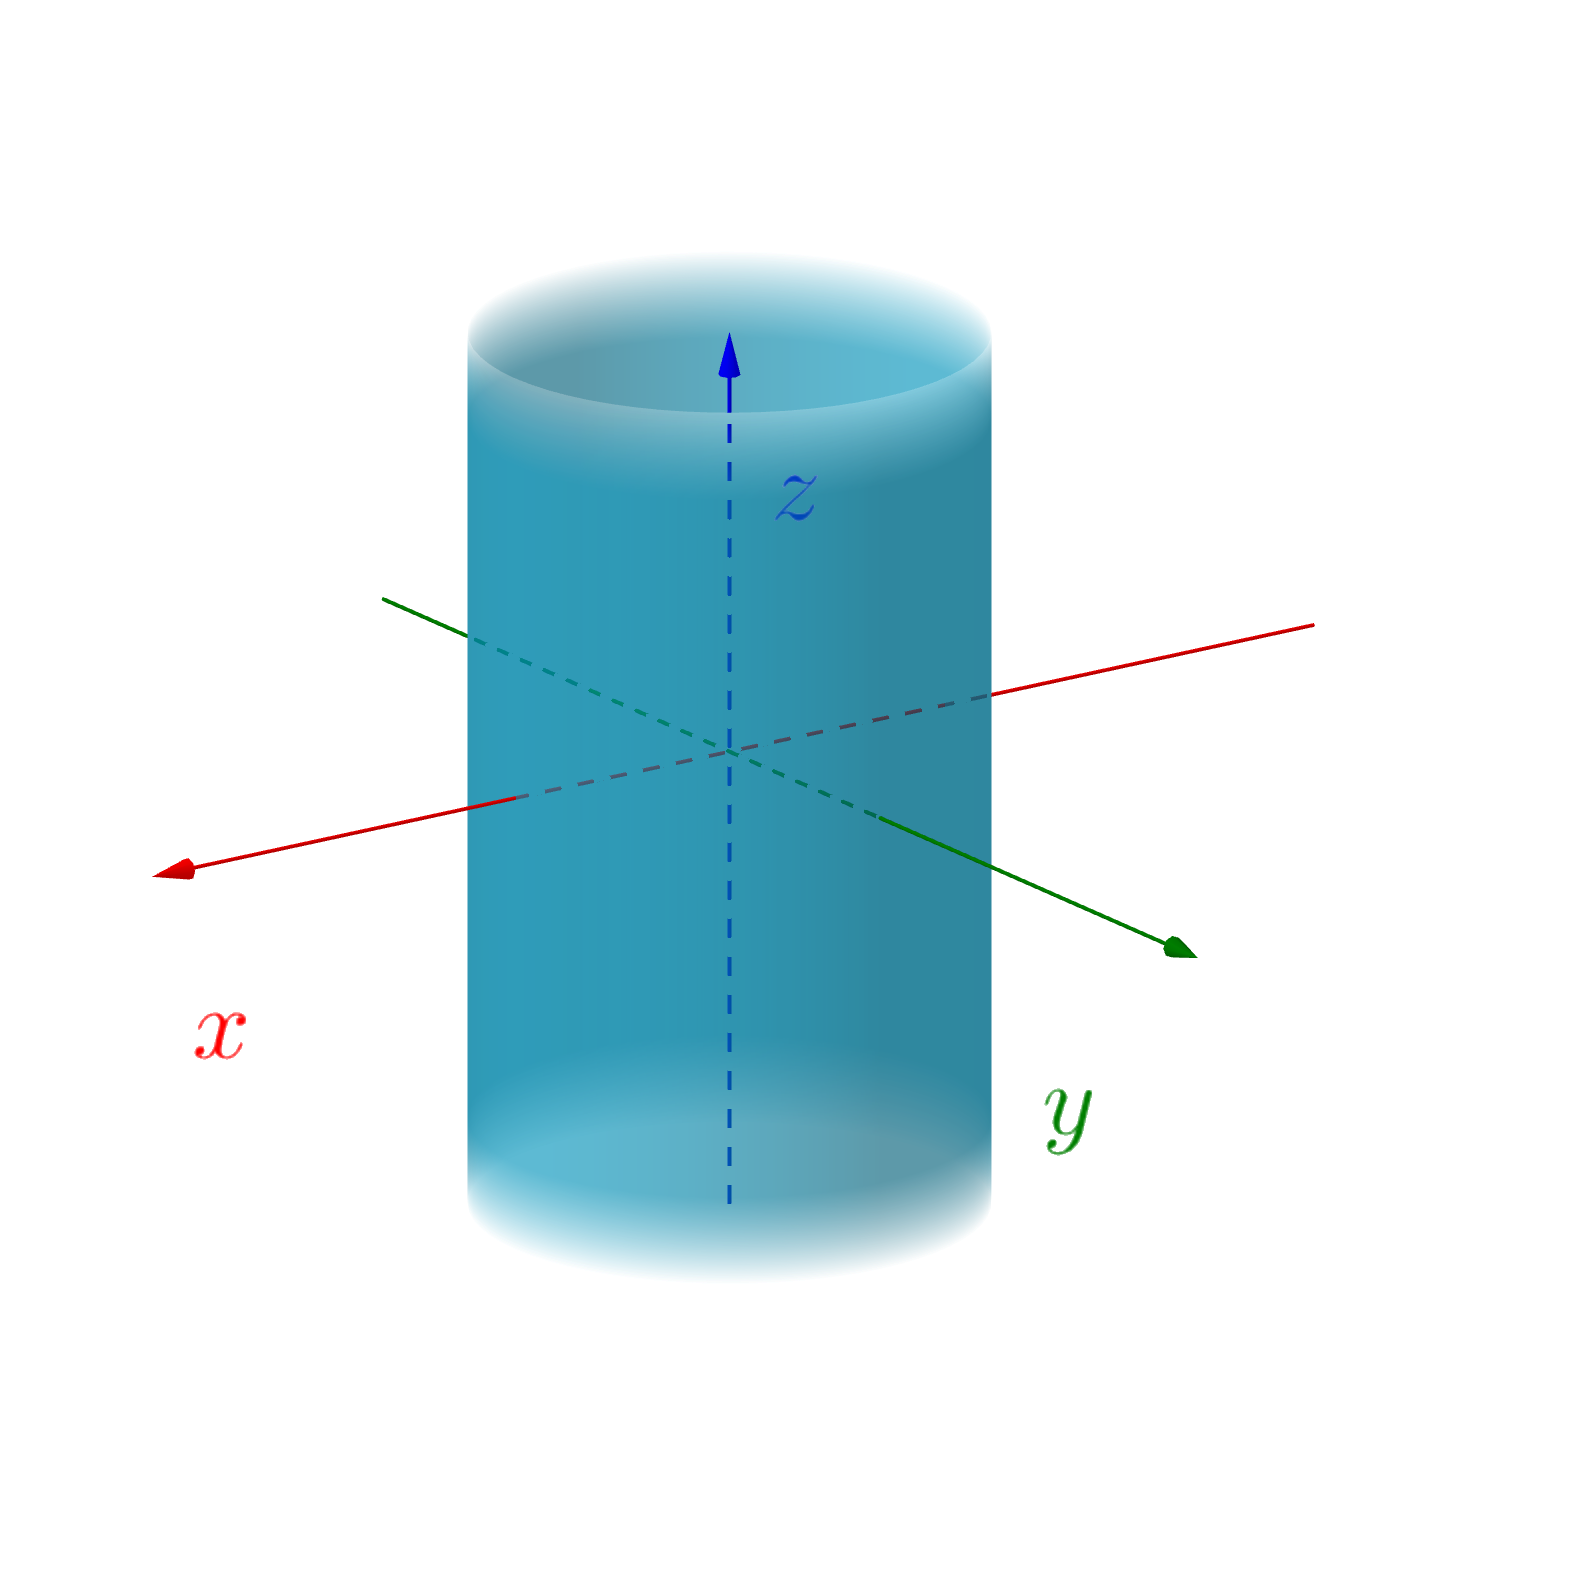
\includegraphics[width=0.9\linewidth]{Plots/e_1_2/1.png} \end{center}
    \end{minipage}

    \item
    \begin{minipage}[t]{0.25\linewidth}
        $\begin{aligned}[t]
            z & = x^2 + y^2 \\
            z & = r^2
        \end{aligned}$
    \end{minipage}
    \begin{minipage}[c]{0.2\linewidth}
        \begin{center}
            \begin{tikzpicture}
                \draw[->] (-1.2, 0) -- (1.2, 0) node[right] {$r_{(y)}$};
                \draw[->] (0, -0.7) -- (0, 1.7) node[above] {$z$};

                \draw[thick,blue,domain=0:1.25] plot (\x, {(\x)^2}) node[above,red] {$z = r^2$};
            \end{tikzpicture}
        \end{center}
    \end{minipage}
    \begin{minipage}[c]{0.5\linewidth}
        \begin{center} 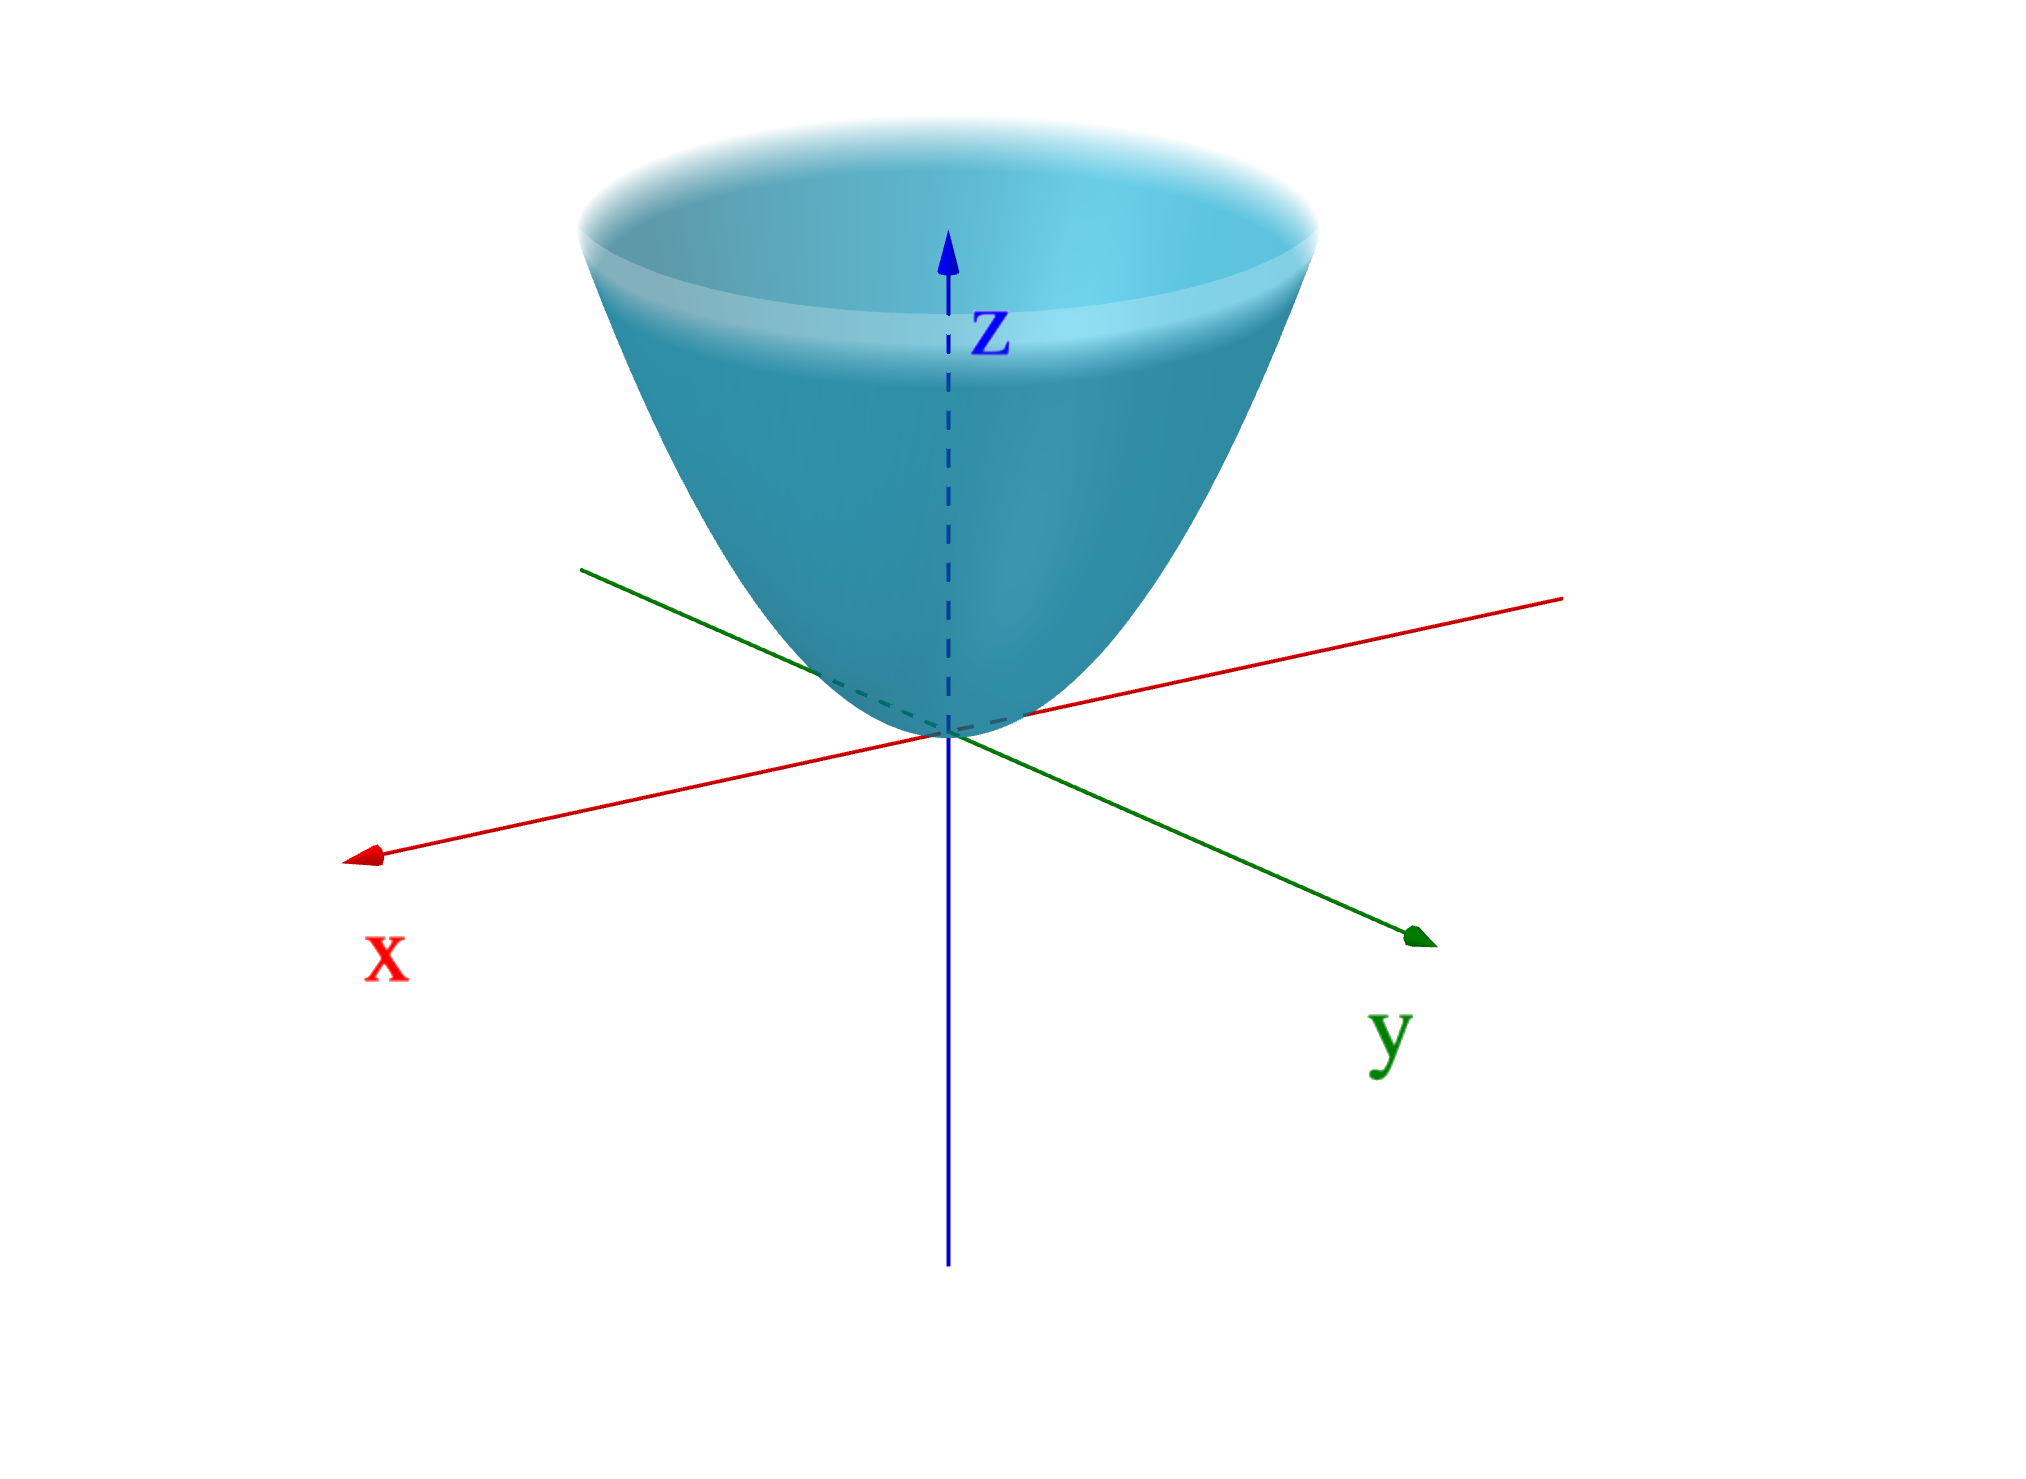
\includegraphics[width=0.9\linewidth]{Plots/e_1_2/2.png} \end{center}
    \end{minipage}

    \item
    \begin{minipage}[t]{0.25\linewidth}
        $\begin{aligned}[t]
            z^2 & = x^2 + y^2 \\
            z^2 & = r^2       \\
            z   & = \pm r
        \end{aligned}$
    \end{minipage}
    \begin{minipage}[c]{0.2\linewidth}
        \begin{center}
            \begin{tikzpicture}
                \draw[->] (-1.2, 0) -- (1.2, 0) node[right] {$r_{(y)}$};
                \draw[->] (0, -1.2) -- (0, 1.2) node[above] {$z$};

                \draw[thick,blue,domain=0:1] plot (\x, {\x});
                \draw[thick,blue,domain=0:1] plot (\x, {-\x});

                \node[red] at (-0.6,0.25) {$z = \pm r$};
            \end{tikzpicture}
        \end{center}
    \end{minipage}
    \begin{minipage}[c]{0.5\linewidth}
        \begin{center} 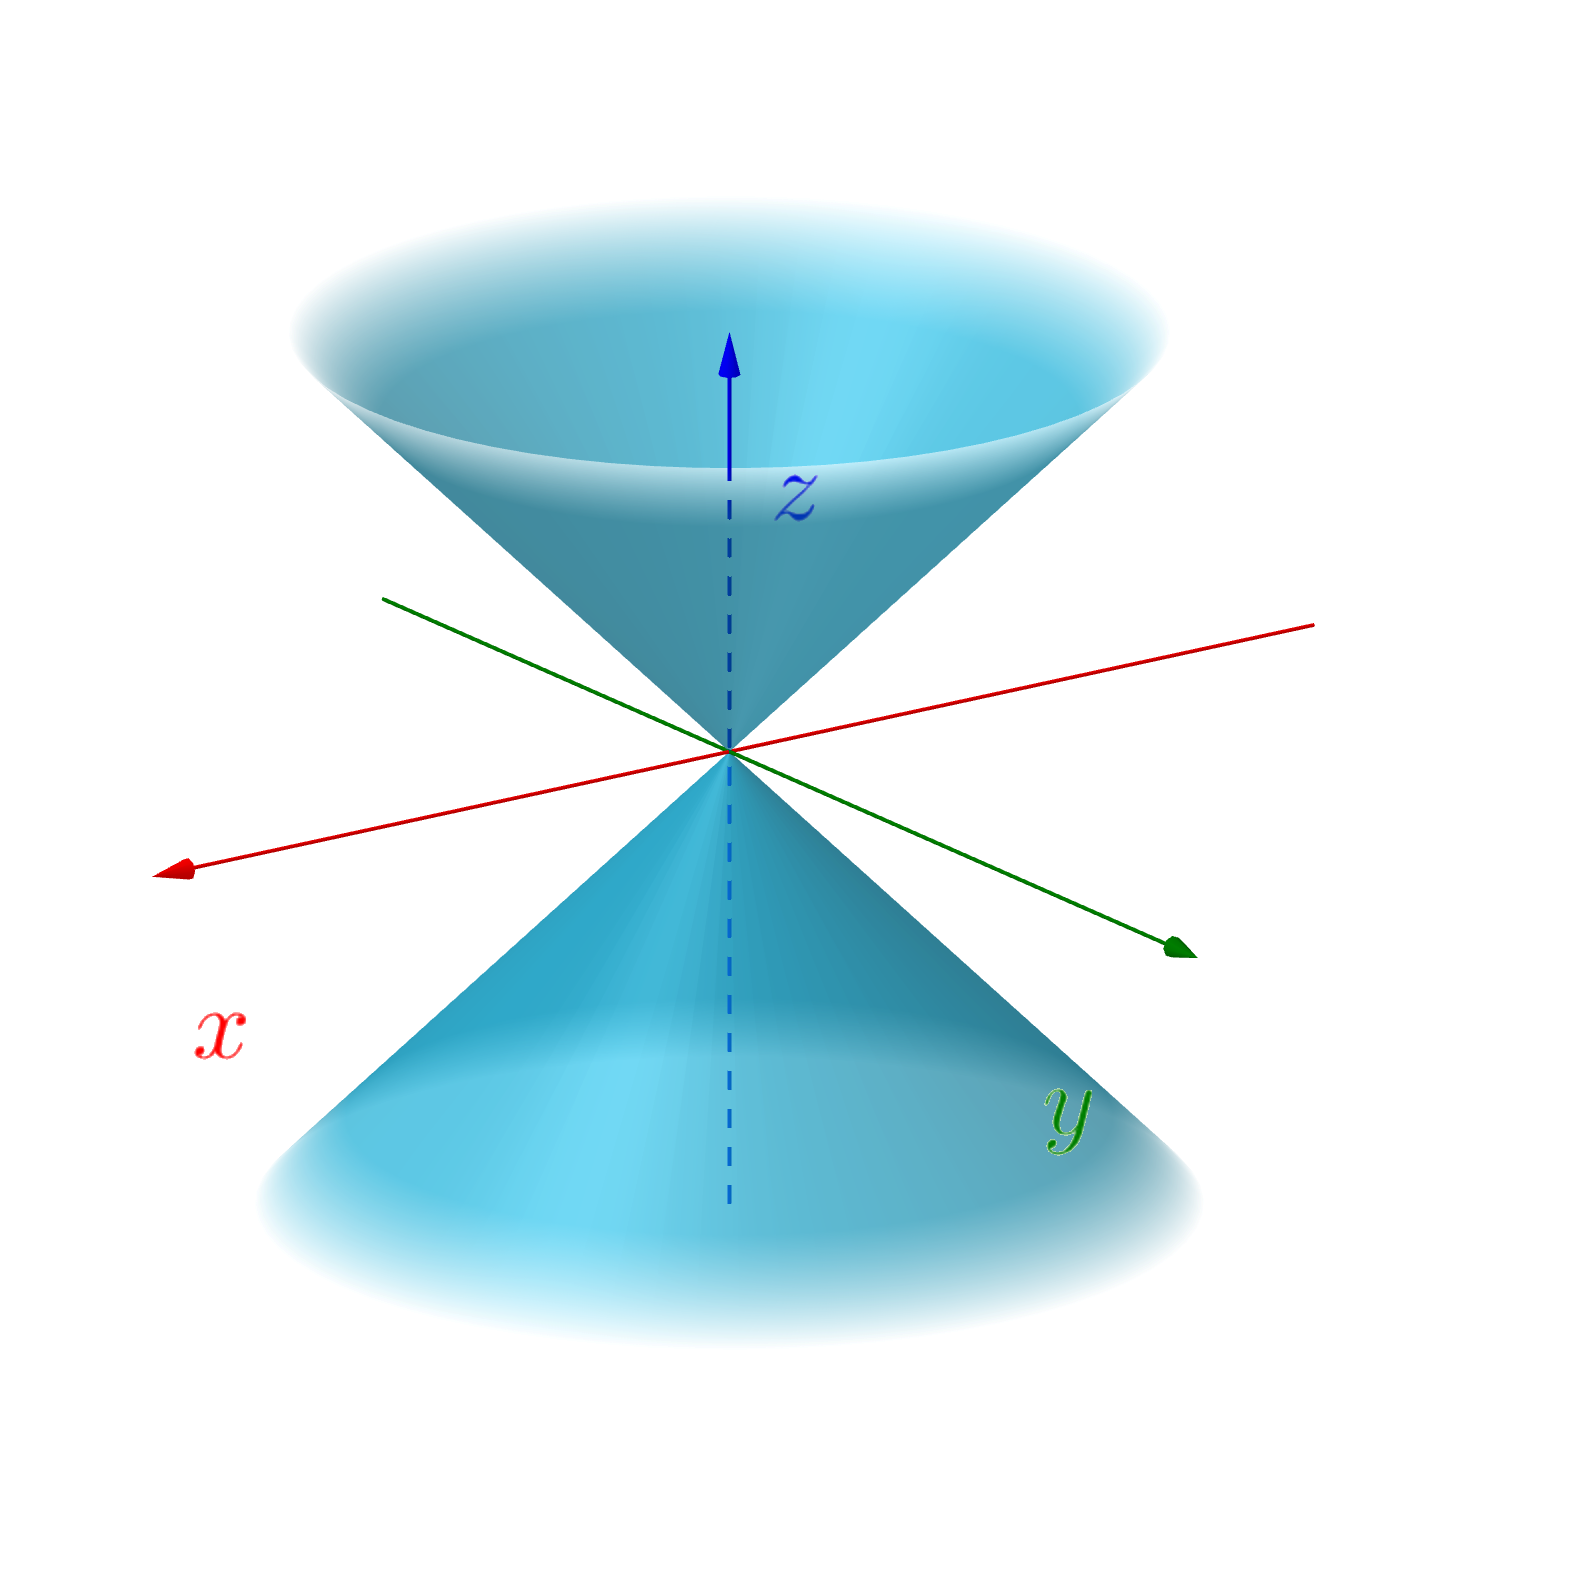
\includegraphics[width=0.9\linewidth]{Plots/e_1_2/3.png} \end{center}
    \end{minipage}

    \item
    \begin{minipage}[t]{0.25\linewidth}
        $\begin{aligned}[t]
            x^2 + y^2 + \frac{z^2}{4}                               & = 1 \\
            r^2 + \frac{z^2}{4}                                     & = 1 \\
            \left(\frac{r}{1}\right)^2 + \left(\frac{z}{2}\right)^2 & = 1
        \end{aligned}$
    \end{minipage}
    \begin{minipage}[c]{0.2\linewidth}
        \begin{center}
            \begin{tikzpicture}
                \draw[->] (-1.2, 0) -- (1.2, 0) node[right] {$r_{(y)}$};
                \draw[->] (0, -1.2) -- (0, 1.2) node[above] {$z$};

                \draw[thick,blue] (0,1) arc (90:-90:0.5cm and 1cm);

                \node[red] at (0,0.5) {$\left(\frac{r}{1}\right)^2 + \left(\frac{z}{2}\right)^2 = 1$};
            \end{tikzpicture}
        \end{center}
    \end{minipage}
    \begin{minipage}[c]{0.5\linewidth}
        \begin{center} 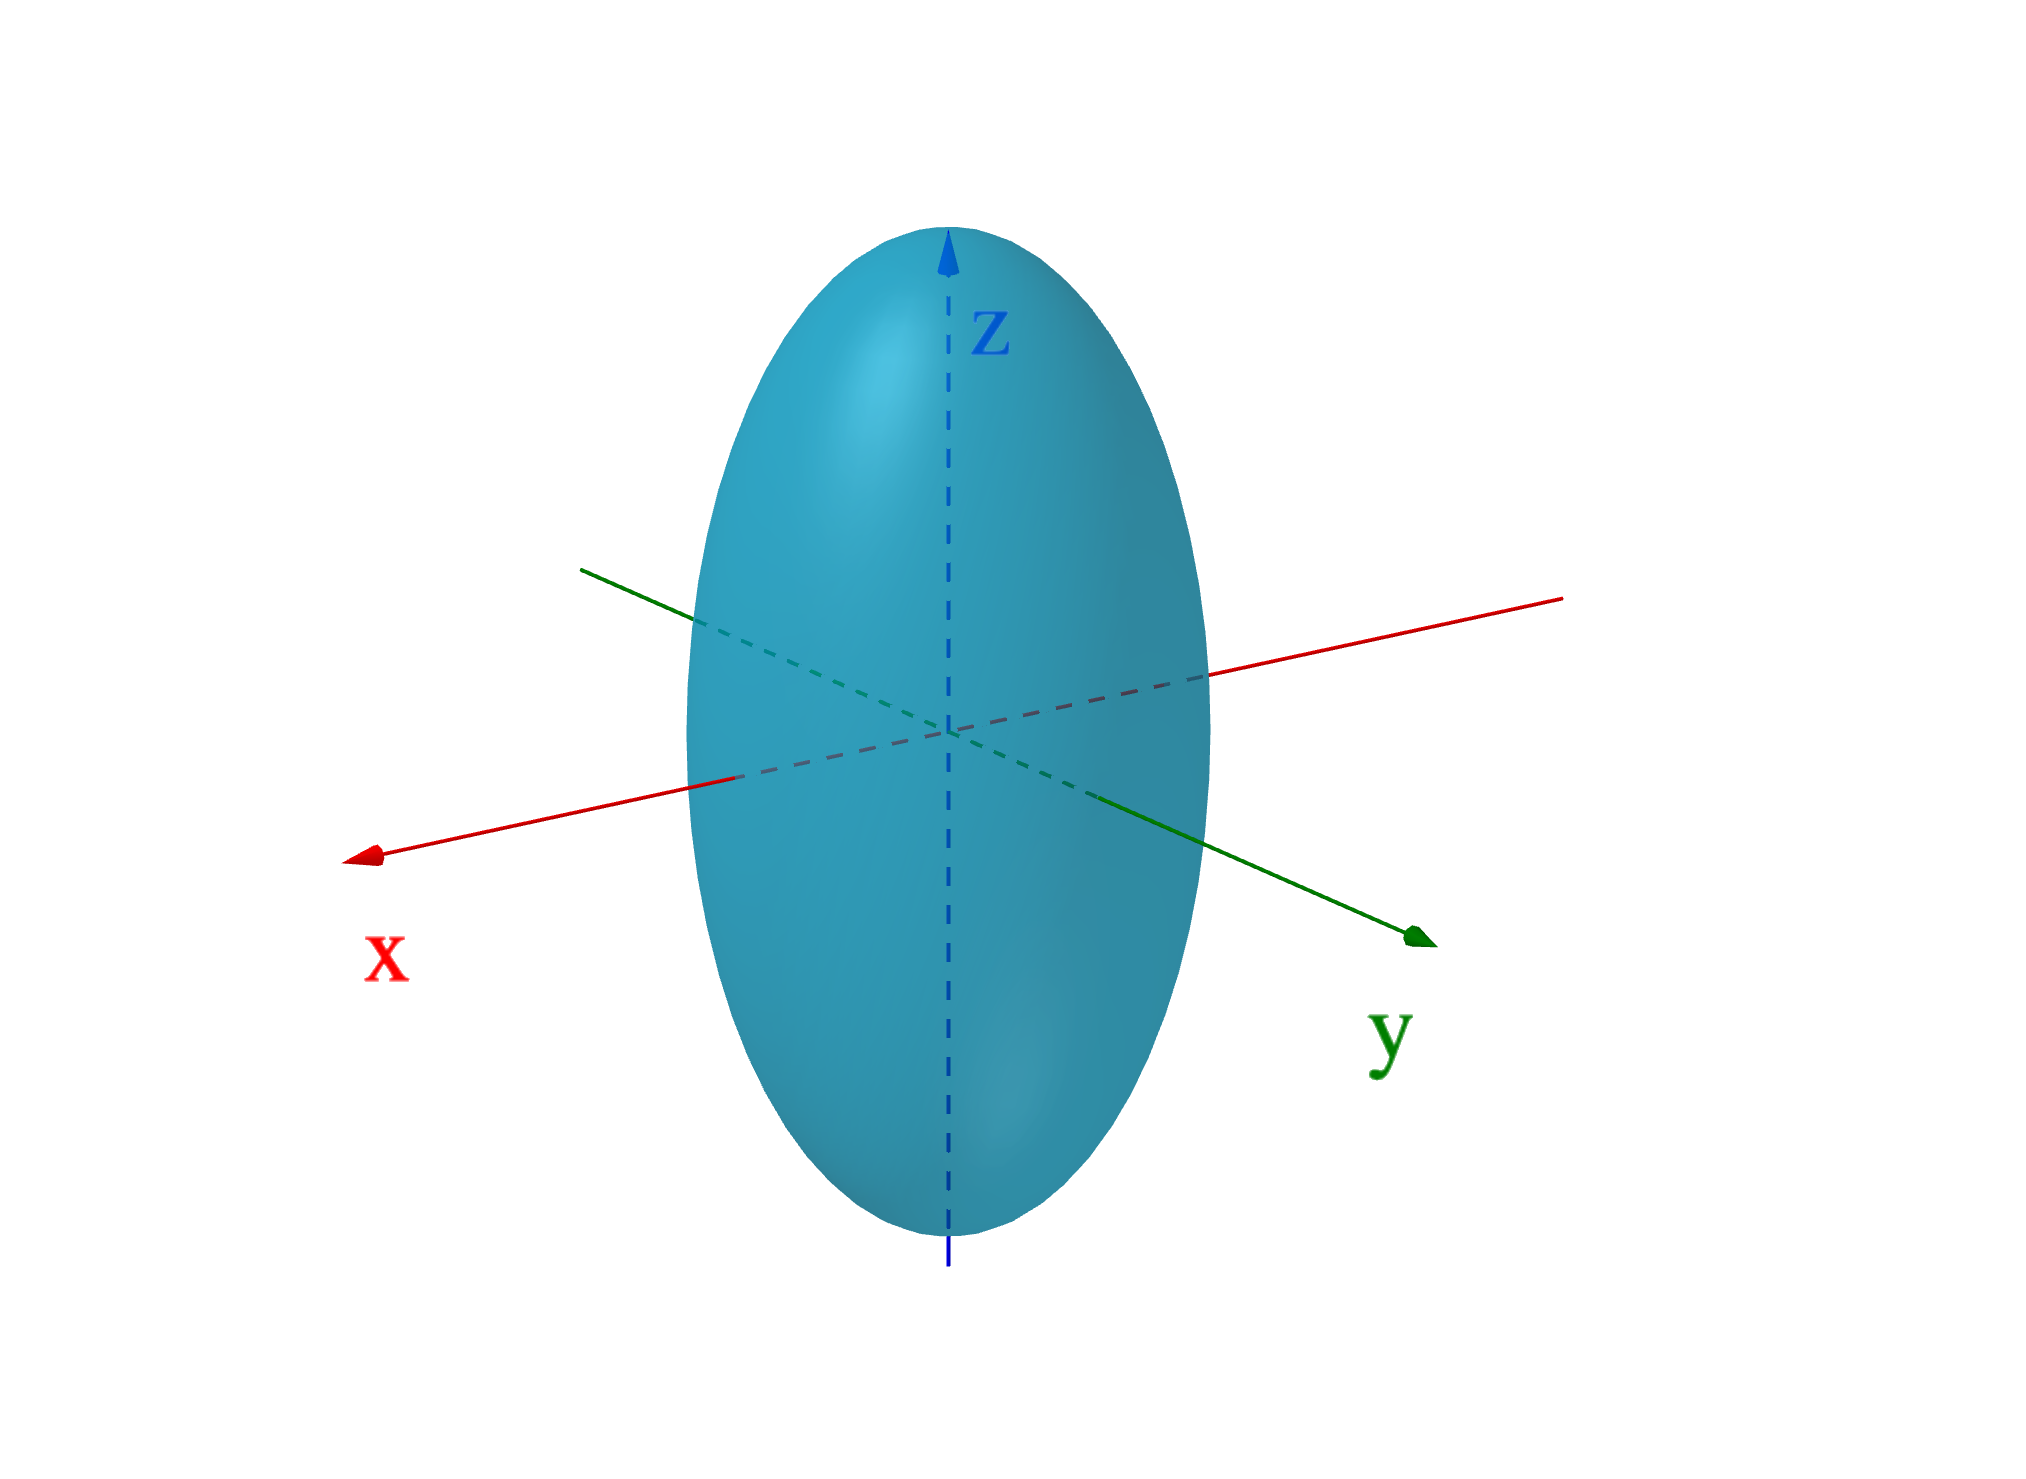
\includegraphics[width=0.9\linewidth]{Plots/e_1_2/4.png} \end{center}
    \end{minipage}

    \item
    \begin{minipage}[t]{0.25\linewidth}
        $\begin{aligned}[t]
            z & = \left(\sqrt{x^2 + y^2} - 1\right)^2 \\
            z & = (r - 1)^2
        \end{aligned}$
    \end{minipage}
    \begin{minipage}[c]{0.2\linewidth}
        \begin{center}
            \begin{tikzpicture}
                \draw[->] (-0.7, 0) -- (1.7, 0) node[right] {$r_{(y)}$};
                \draw[->] (0, -0.7) -- (0, 1.7) node[above] {$z$};

                \draw[thick,blue,domain=0:2.5] plot (\x, {(\x - 1)^2}) node[below left,red] {$z = (r - 1)^2$};
            \end{tikzpicture}
        \end{center}
    \end{minipage}
    \begin{minipage}[c]{0.5\linewidth}
        \begin{center} 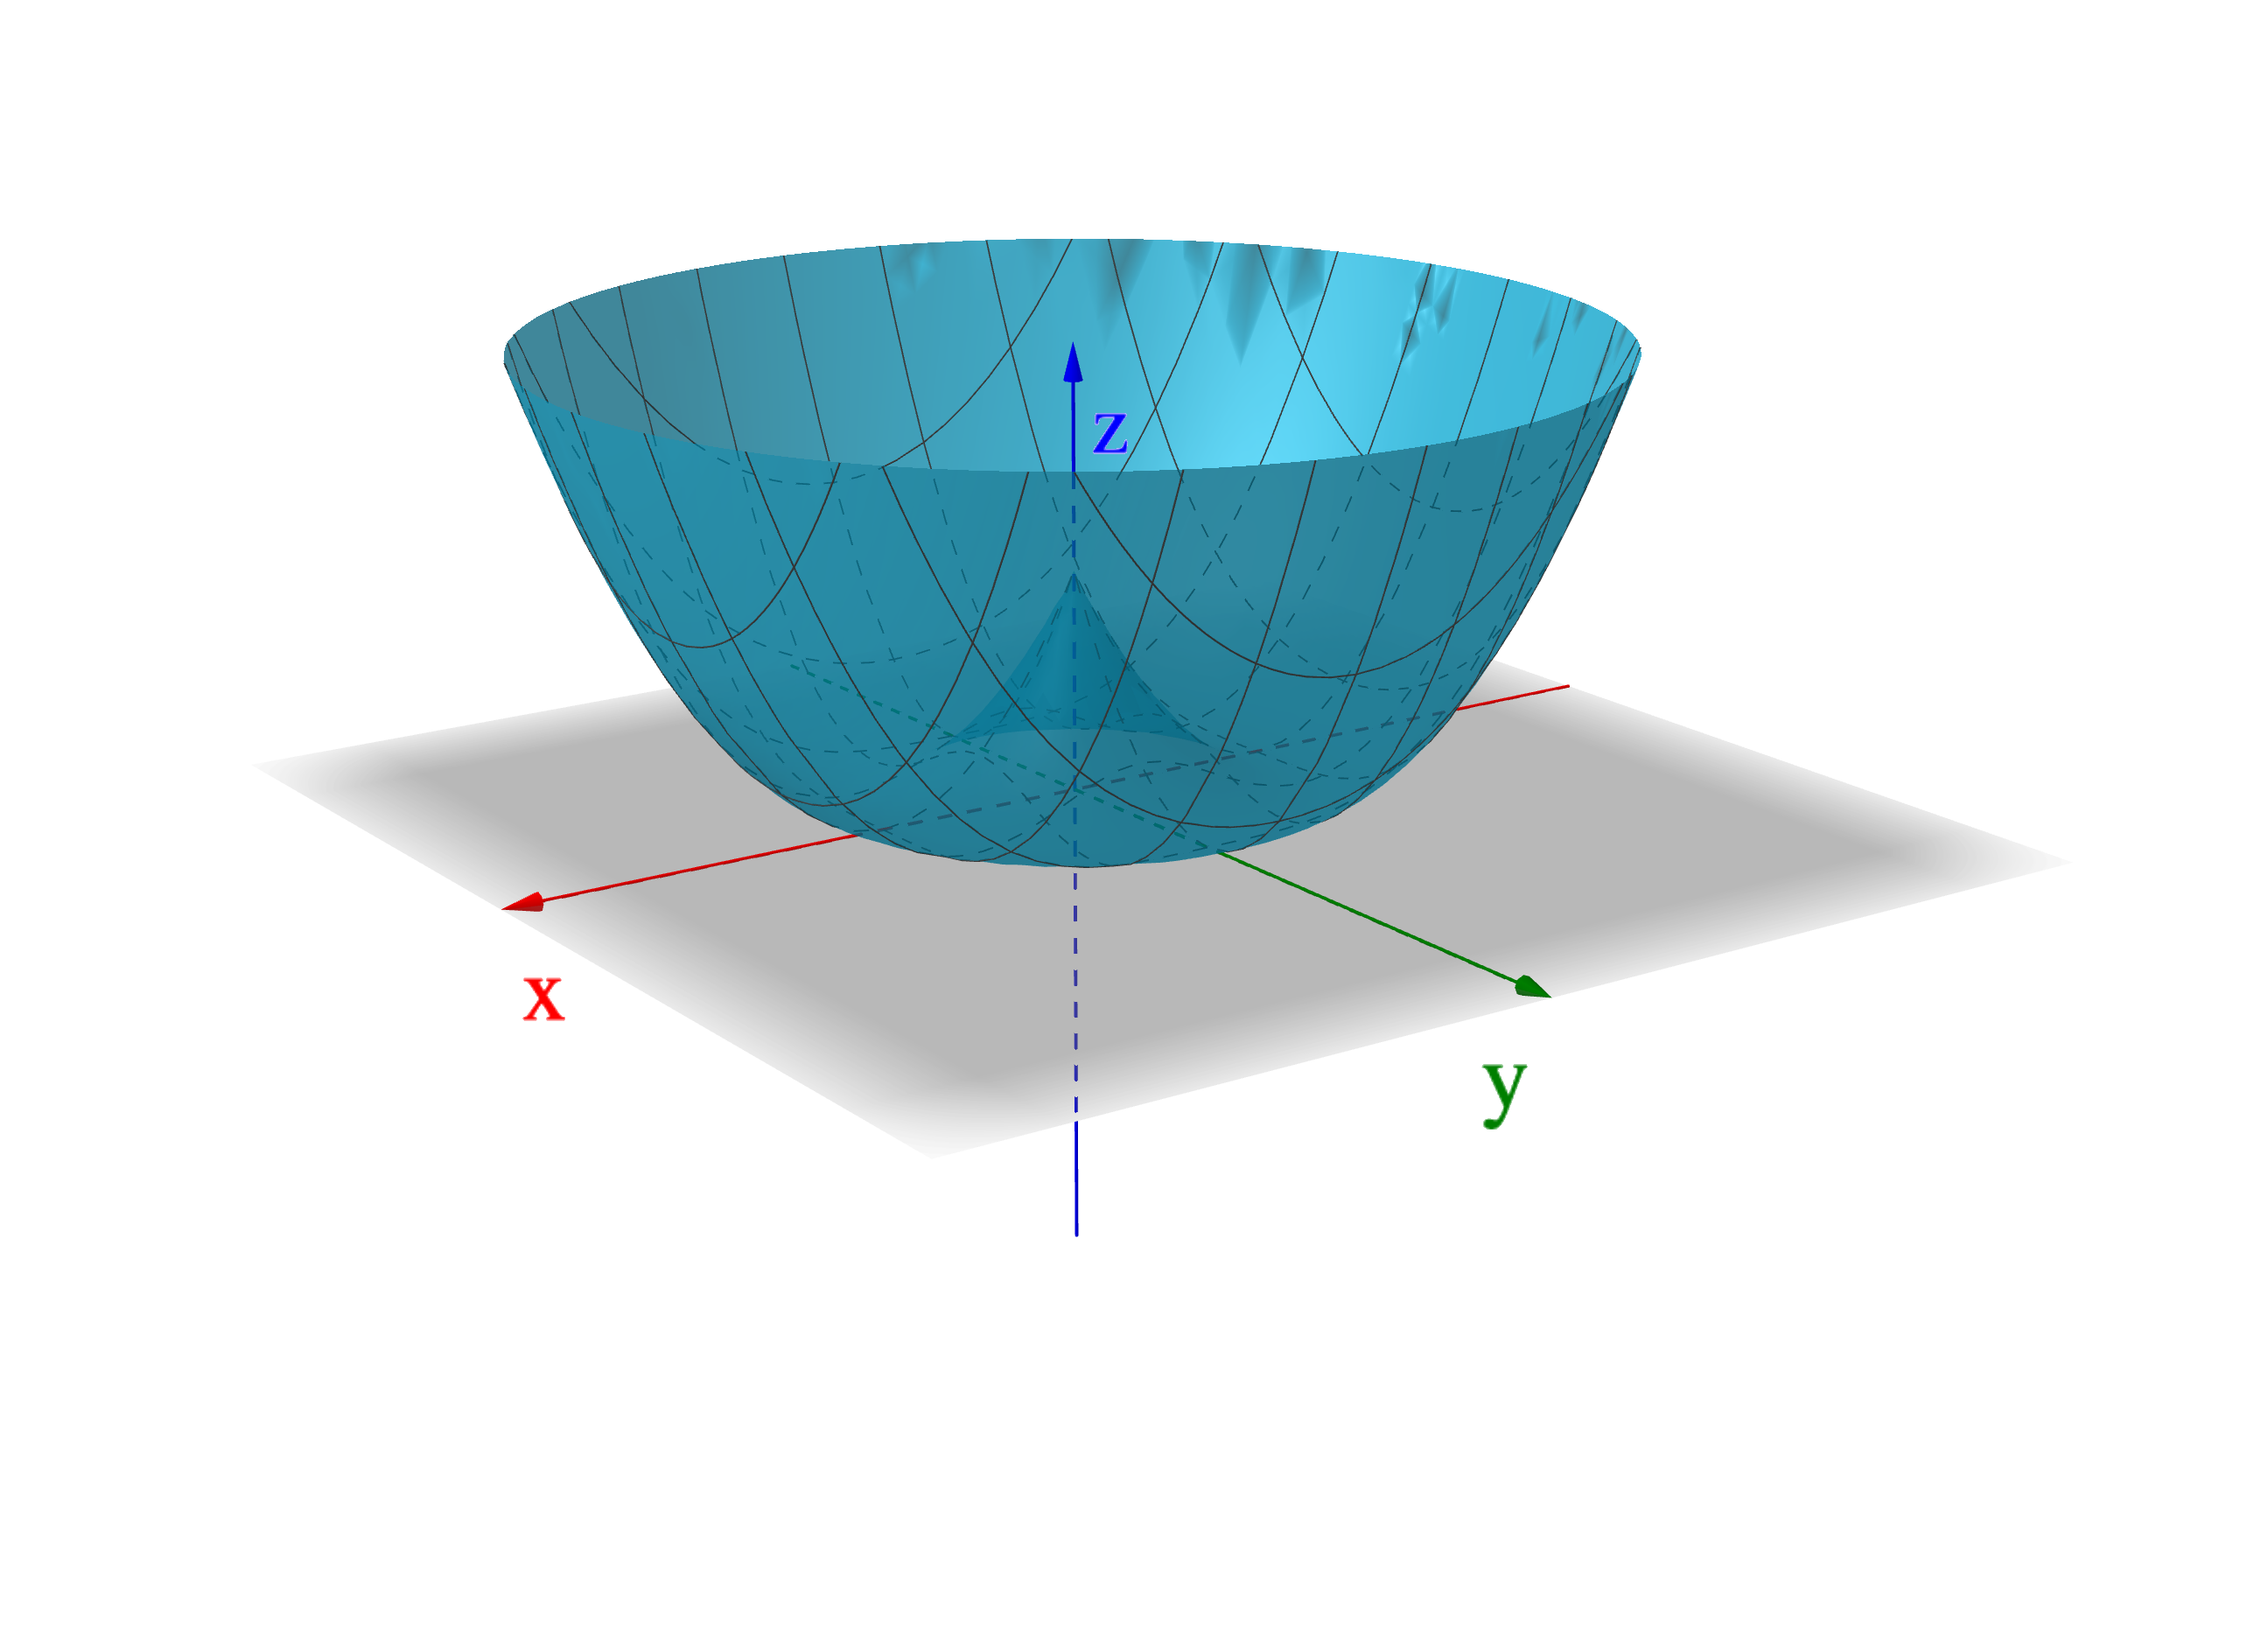
\includegraphics[width=0.9\linewidth]{Plots/e_1_2/5.png} \end{center}
    \end{minipage}

    \item
    \begin{minipage}[t]{0.25\linewidth}
        $\begin{aligned}[t]
            x^2 + y^2 + z^2    & = 2z \\
            r^2 + z^2 - 2z + 1 & = 1  \\
            r^2 + (z - 1)^2    & = 1
        \end{aligned}$
    \end{minipage}
    \begin{minipage}[c]{0.2\linewidth}
        \begin{center}
            \begin{tikzpicture}
                \draw[->] (-1.2, 0) -- (1.2, 0) node[right] {$r_{(y)}$};
                \draw[->] (0, -0.2) -- (0, 2.2) node[above] {$z$};

                \draw[thick,blue] (0,2) arc (90:-90:1cm and 1cm);

                \node[red] at (0,1) {$r^2 + (z - 1)^2 = 1$};
            \end{tikzpicture}
        \end{center}
    \end{minipage}
    \begin{minipage}[c]{0.5\linewidth}
        \begin{center} 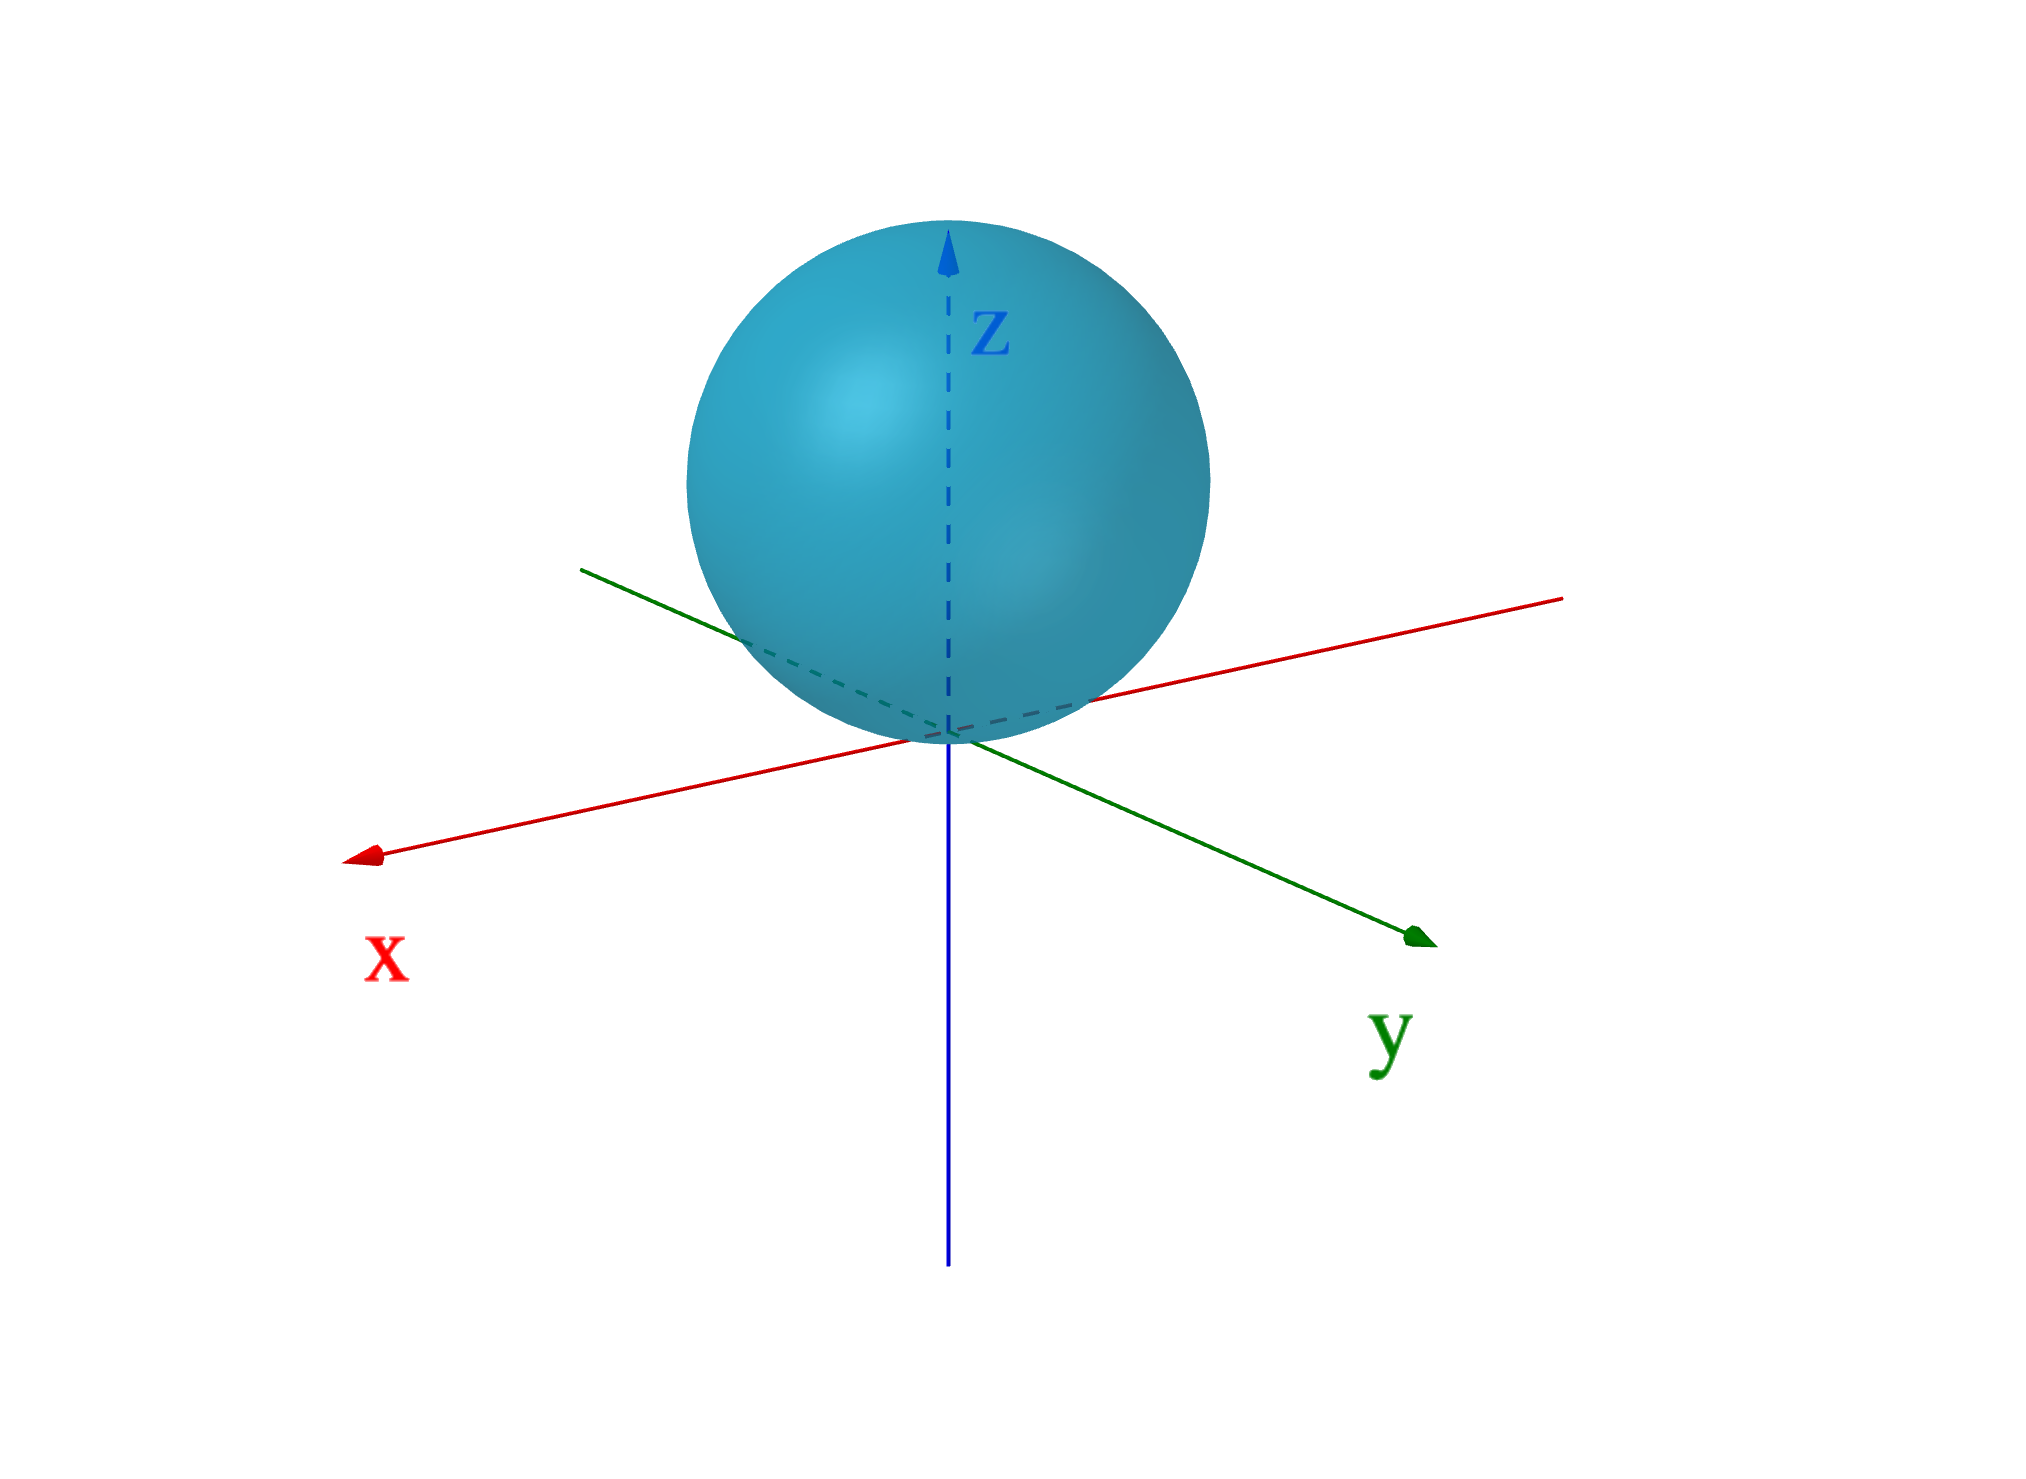
\includegraphics[width=0.9\linewidth]{Plots/e_1_2/6.png} \end{center}
    \end{minipage}
\end{enumerate}

\section*{Chapter 2}

\subsection*{Exercise 2.1}

\begin{enumerate}
    \item 
    $\begin{aligned}[t]
        \det \begin{pmatrix} 3 & -1 \\ 2 & 5 \end{pmatrix} 
        & = 3 \times 5 - 2 \times (-1) \\
        & = 15 + 2                     \\
        & = 17
    \end{aligned}$

    {~~~}

    \item 
    $\begin{aligned}[t]
        \det \begin{pmatrix} 1 & 3 & -3 \\ -3 & -5 & 2 \\ -4 & 4 & -6 \end{pmatrix}
        & = 1 \cdot \det \begin{pmatrix} -5 & 2 \\ 4 & -6 \end{pmatrix} - 3 \cdot \det \begin{pmatrix} -3 & 2 \\ -4 & -6 \end{pmatrix} + (-3) \cdot \det \begin{pmatrix} -3 & -5 \\ -4 & 4 \end{pmatrix} \\
        & = 1 \cdot 22 - 3 \cdot 26 + (-3) \cdot (-32)                  \\
        & = 22 - 78 + 96                                                \\
        & = 40
    \end{aligned}$

    {~~~}

    \item 
    $\begin{aligned}[t]
        \det \begin{pmatrix} 3 & 1 & 0 \\ 1 & 3 & 4 \\ 0 & 0 & 4 \end{pmatrix} & = 0 \cdot \det \begin{pmatrix} 1 & 0 \\ 3 & 4 \end{pmatrix} - 0 \cdot \det \begin{pmatrix} 3 & 0 \\ 1 & 4 \end{pmatrix} + 4 \cdot \det \begin{pmatrix} 3 & 1 \\ 1 & 3 \end{pmatrix}
        & \text{since }\begin{pmatrix} + & - & + \\ - & + & - \\ + & - & + \end{pmatrix}             \\
                                                                               & = 0 - 0 + 4 \cdot 8 \\
                                                                               & = 32
    \end{aligned}$
\end{enumerate}

\subsection*{Exercise 2.2}

\begin{minipage}[t]{0.45\linewidth}
    \begin{enumerate}
        \item 
        $\begin{aligned}[t]
            | \vec{a} |           & = \sqrt{\vec{a} \cdot \vec{a}}                          \\
                                  & = \sqrt{4^2 + 3^2}                                      \\
                                  & = 5
            \\ \\
            | \vec{b} |           & = \sqrt{\vec{b} \cdot \vec{b}}                          \\
                                  & = \sqrt{2^2 + (-1)^2}                                   \\
                                  & = \sqrt{5}
            \\ \\
            \vec{a} \cdot \vec{b} & = 4 \cdot 2 + 3 \cdot (-1)                              \\
                                  & = 5
            \\ \\
            \vec{a} \cdot \vec{b} & = | \vec{a} | | \vec{b} | \cos(\theta)                  \\
            \cos \theta           & = \frac{\vec{a} \cdot \vec{b}}{| \vec{a} | | \vec{b} |} \\
                                  & = \frac{5}{5 \cdot \sqrt{5}}                            \\
            \theta                & = \arccos \left( \frac{1}{\sqrt{5}} \right)
        \end{aligned}$
    \end{enumerate}
\end{minipage}
\begin{minipage}[t]{0.45\linewidth}
    \begin{enumerate} \setcounter{enumi}{1}
        \item 
        $\begin{aligned}[t]
            | \vec{a} |           & = \sqrt{\vec{a} \cdot \vec{a}}                          \\
                                  & = \sqrt{4^2 + 0^2 + 2^2}                                \\
                                  & = 2\sqrt{5}
            \\ \\
            | \vec{b} |           & = \sqrt{\vec{b} \cdot \vec{b}}                          \\
                                  & = \sqrt{2^2 + (-1)^2 + 0^2}                             \\
                                  & = \sqrt{5}
            \\ \\
            \vec{a} \cdot \vec{b} & = 4 \cdot 2 + 0 \cdot (-1) + 2 \cdot 0                  \\
                                  & = 8
            \\ \\
            \vec{a} \cdot \vec{b} & = | \vec{a} | | \vec{b} | \cos(\theta)                  \\
            \cos \theta           & = \frac{\vec{a} \cdot \vec{b}}{| \vec{a} | | \vec{b} |} \\
                                  & = \frac{8}{2\sqrt{5} \cdot \sqrt{5}}                    \\
            \theta                & = \arccos \left( \frac{4}{5} \right)
        \end{aligned}$
    \end{enumerate}
\end{minipage}

\vfill
\subsection*{Exercise 2.3}

$\begin{aligned}[t]
    \vec{x} \times \vec{y} 
    & = \det \begin{pmatrix} i & j & k \\ 3 & -2 & 1 \\ 1 & -1 & 1 \end{pmatrix} \\
    & = i \cdot \det \begin{pmatrix} -2 & 1 \\ -1 & 1 \end{pmatrix} - j \cdot \det \begin{pmatrix} 3 & 1 \\ 1 & 1 \end{pmatrix} + k \cdot \begin{pmatrix} 3 & -2 \\ 1 & -1 \end{pmatrix} \\
    & = (-1, -2, -1)
\end{aligned}$

\subsection*{Exercise 2.4}

\begin{enumerate}
    \item
    $\begin{aligned}[t]
        \vec{v} 
        & =(3, -2, 4) - (-8, 0, 4)                                                                   \\
        & = (11, -2, 0)
        \\
        \vec{r} 
        & = t\begin{bmatrix} 11 \\ 2 \\ 0 \end{bmatrix} + \begin{bmatrix} -8 \\ 0 \\ 4 \end{bmatrix}
    \end{aligned}$

    {~~~}

    \item
    $\begin{cases}
        \vec{r}_0 = (0, 0, 0) \\
        \vec{n} = (1, 5, 2)
    \end{cases}$

    {~~~}

    $\begin{aligned}[t]
        \vec{n} \cdot \vec{r}                                   
        & = \vec{n} \cdot \vec{r}_0                                                                   \\
        \begin{bmatrix} 1 \\ 5 \\ 2 \end{bmatrix} \cdot \vec{r} 
        & = \begin{bmatrix} 1 \\ 5 \\ 2 \end{bmatrix} \cdot \begin{bmatrix} 0 \\ 0 \\ 0 \end{bmatrix} \\
        \begin{bmatrix} 1 \\ 5 \\ 2 \end{bmatrix} \cdot \vec{r} 
        & = 0
    \end{aligned}$

    {~~~}

    \item
    $\begin{cases}
        \vec{r}_0 = (2, 4, 6) \\
        \vec{n} ~= (1, 1, -1)
    \end{cases}$

    {~~~}

    $\begin{aligned}[t]
        \vec{n} \cdot \vec{r}                                    
        & = \vec{n} \cdot \vec{r}_0                                                                     \\
        \begin{bmatrix} 1 \\ 1 \\ -1 \end{bmatrix} \cdot \vec{r} 
        & = \begin{bmatrix} 1 \\ 1 \\ -1 \end{bmatrix} \cdot \begin{bmatrix} 2 \\ 4 \\ -6 \end{bmatrix} \\
        \begin{bmatrix} 1 \\ 1 \\ -1 \end{bmatrix} \cdot \vec{r} & = 0
    \end{aligned}$

    {~~~}

    \item
    $\vec{x} = (1, 0, 1) - (0, 1, 1) = (1, -1, 0)$, and $\vec{y} = (1, 1, 0) - (0, 1, 1) = (1, 0, -1)$.

    {~~~}

    $\begin{aligned}[t]
        \vec{n}
        & = \vec{x} \times \vec{y}\\
        & = \det \begin{pmatrix} i & j & k \\ 1 & -1 & 0 \\ 1 & 0 & -1 \end{pmatrix} \\
        & = i \cdot \det \begin{pmatrix} -1 & 0 \\ 0 & -1 \end{pmatrix} - j \cdot \det \begin{pmatrix} 1 & 0 \\ 1 & -1 \end{pmatrix} + k \cdot \det \begin{pmatrix} 1 & -1 \\ 1 & 0 \end{pmatrix} \\
        & = \begin{bmatrix} 1 \\ 1 \\ 1 \end{bmatrix}
    \end{aligned}$

    $\begin{cases}
        \vec{r}_0 = (0, 1, 1) \\
        \vec{n} ~= (1, 1, 1)
    \end{cases}$

    {~~~}

    $\begin{aligned}[t]
        \vec{n} \cdot \vec{r}
        & = \vec{n} \cdot \vec{r}_0                                                                   \\
        \begin{bmatrix} 1 \\ 1 \\ 1 \end{bmatrix} \cdot \vec{r}
        & = \begin{bmatrix} 1 \\ 1 \\ 1 \end{bmatrix} \cdot \begin{bmatrix} 0 \\ 1 \\ 1 \end{bmatrix} \\
        \begin{bmatrix} 1 \\ 1 \\ 1 \end{bmatrix} \cdot \vec{r}
        & = 0
    \end{aligned}$

    {~~~}

    \item 
    $\begin{aligned}[t]
        \vec{r}_0 & = \frac{(3, 1, 5) + (-2, 0, 0)}{2} \\
                  & = \frac{1}{2} (1, 1, 5)
        \\ \\
        \vec{n}   & = (-2, 0, 0) - (3, 1, 5)           \\
                  & = (-5, -1, -5)
    \end{aligned}$

    {~~~}

    {~~~}

    $\begin{aligned}[t]
        \vec{n} \cdot \vec{r}     & = \vec{n} \cdot \vec{r}_0                \\
        (-5, 1, -5) \cdot \vec{r} & = (-5, 1, -5) \cdot \frac{1}{2}(1, 1, 5) \\
        -5x - y - 5z              & = \frac{1}{2}(-5 + 1 - 25)               \\
                                  & = \frac{-31}{2}
    \end{aligned}$
\end{enumerate}

\section*{Chapter 3}

\subsection*{Exercise 3.1}

\begin{enumerate}
    \item 
    \begin{minipage}[t]{0.45\linewidth}
        At $k = 2$, 
        $\begin{aligned}[t]
            4x^2 + y^2 + 1 &= 2 \\
            4x^2 + y^2     &= 1 \\
            \left(\frac{x}{\frac{1}{2}}\right)^2 + \left(\frac{y}{1}\right)^2 &= 1
        \end{aligned}$
    \end{minipage}
    \begin{minipage}[t]{0.45\linewidth}
        At $k = 5$, 
        $\begin{aligned}[t]
            4x^2 + y^2 + 1      &= 5 \\
            4x^2 + y^2          &= 4 \\
            x^2 + \frac{y^2}{4} &= 1 \\
            \left(\frac{x}{1}\right)^2 + \left(\frac{y}{2}\right)^2 &= 1
        \end{aligned}$
    \end{minipage}

    \begin{center}
        \begin{tikzpicture}
            \draw[->] (-2.2,0) -- (2.2,0) node[right] {$x$};
            \draw[->] (0,-2.7) -- (0,2.7) node[above] {$y$};
            
            \draw[thick,blue] (0,0) ellipse (0.5cm and 1cm);
            \draw[thick,DarkGreen] (0,0) ellipse (1cm and 2cm);

            \draw[thick,red] (0.5,0.25) -- (0.5,0) node[below left] {$\frac{1}{2}$};
            \draw[thick,red] (1,0.25) -- (1,0) node[below left] {$1$};

            \draw[thick,red] (0.25,1) -- (0,1) node[left] {$1$};
            \draw[thick,red] (0.25,2) -- (0,2) node[left] {$2$};

            \node[blue] at (1.5,3) {Level set at $k = 2$};
            \node[DarkGreen] at (1.5,2.5) {Level set at $k = 5$};
        \end{tikzpicture}
    \end{center}

    \item 
    \begin{minipage}[t]{0.45\linewidth}
        At $k = 0$, 
        $\begin{aligned}[t]
            x^2 + y^2 - z &= 0 \\
            x^2 + y^2     &= z \\
            r^2           &= z
        \end{aligned}$
        
        \begin{center} 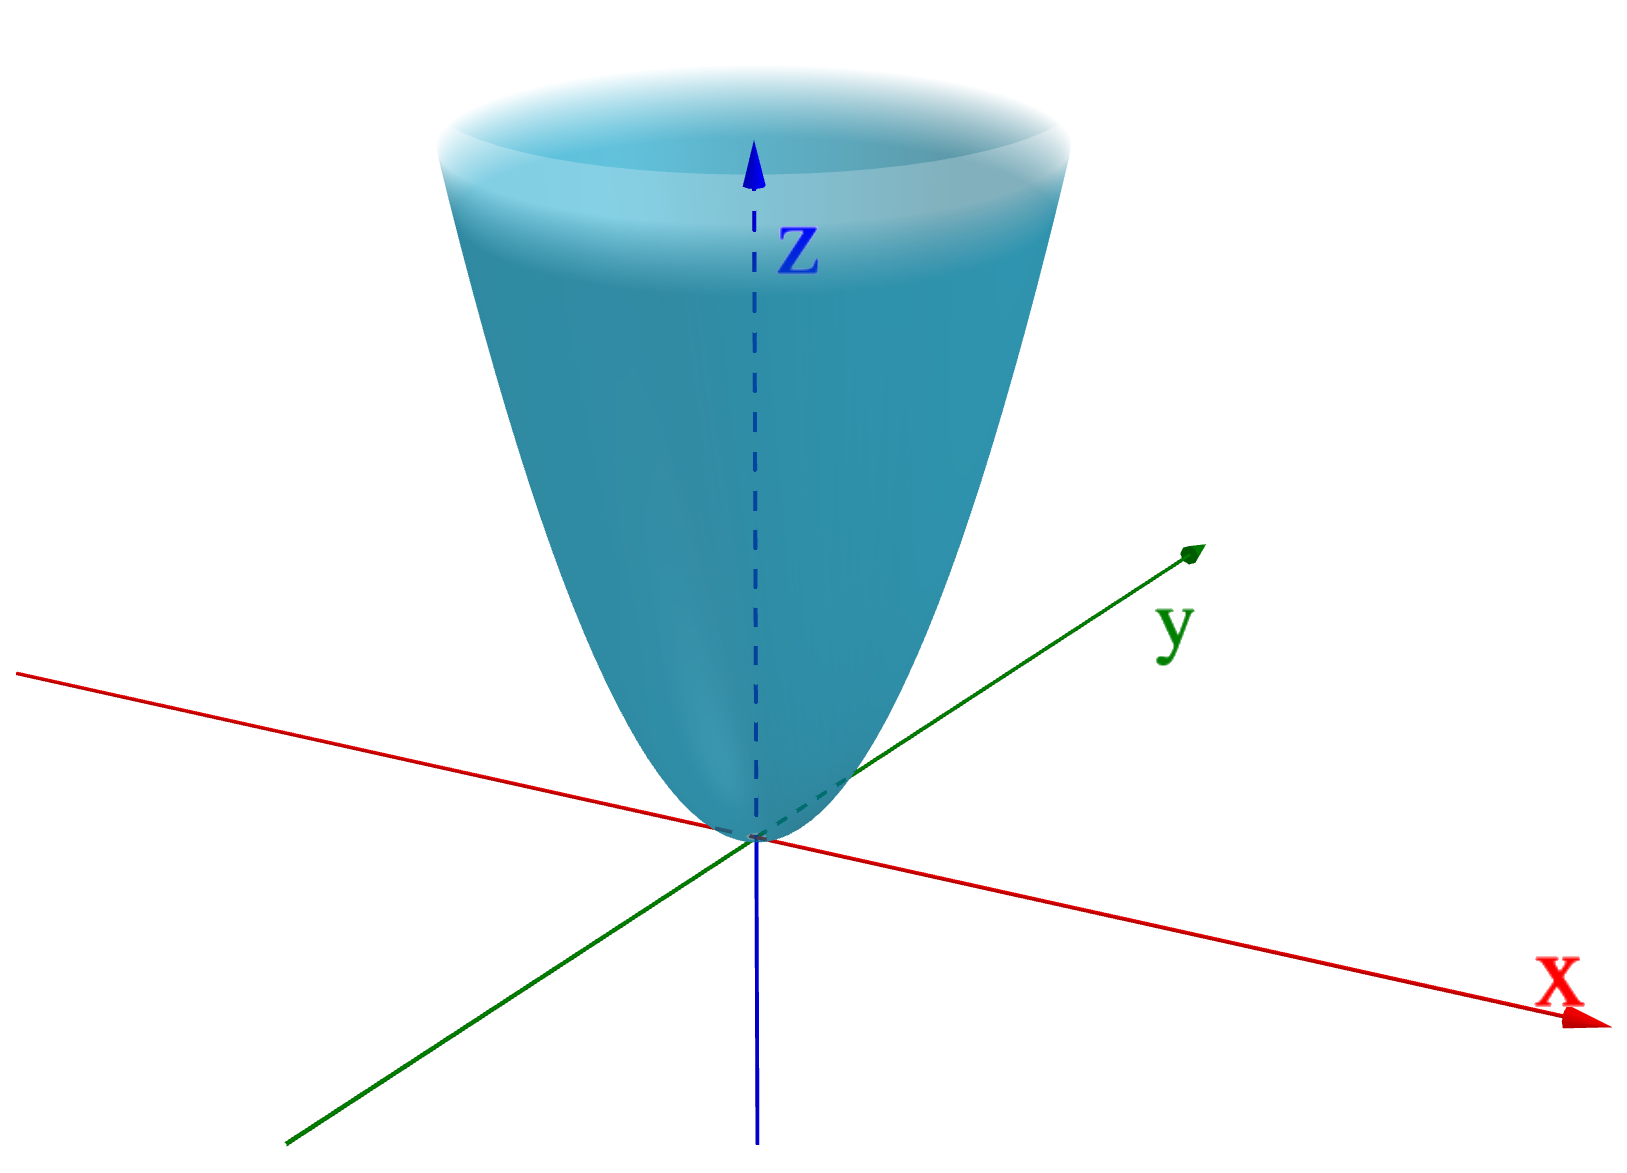
\includegraphics[width=\linewidth]{Plots/e_1_7/1.png} \end{center}
    \end{minipage}
    \begin{minipage}[t]{0.45\linewidth}
        At $k = 2$, 
        $\begin{aligned}[t]
            x^2 + y^2 - z &= 2 \\
            x^2 + y^2 - 2 &= z \\
            r^2 - 2       &= z
        \end{aligned}$

        \begin{center} 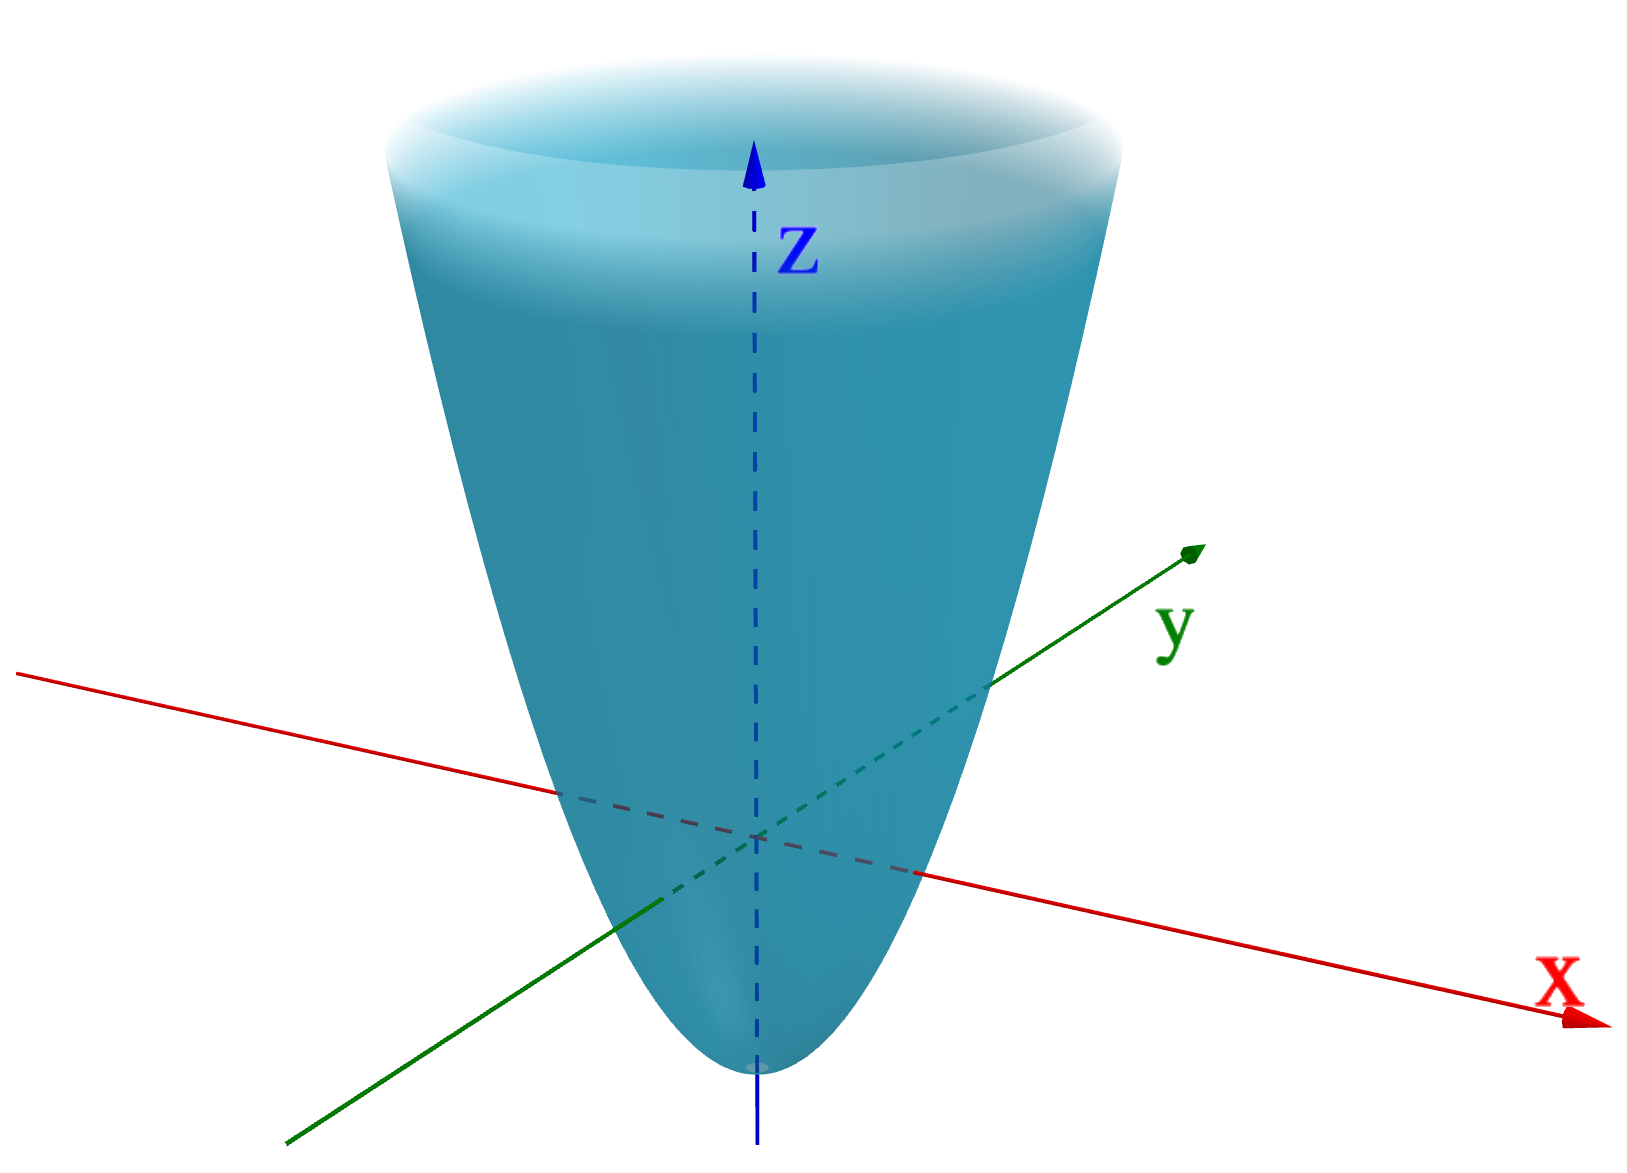
\includegraphics[width=\linewidth]{Plots/e_1_7/2.png} \end{center}
    \end{minipage}
\end{enumerate}

\subsection*{Exercise 3.2}

\begin{itemize}
        \item For $x = 0$, $\lim_{(x,y)\to(0,0)}f(x,y) = \lim_{y\to0}\frac{0}{0 + y^2} = 0$. 

        {~~~}

        \item For $y = x$, $\lim_{(x,y)\to(0,0)}f(x,y) = \lim_{x\to0} \frac{x^2x}{x^4 + x^2} = \lim_{x\to0} \frac{x}{x+1} = 0$. 

        {~~~}

        \item For $y = 0$, $\lim_{(x,y)\to(0,0)}f(x,y) = \lim_{x\to0}\frac{0}{x^4 + 0} = 0$. 

        {~~~}

        \item For $y = x^2$, $\lim_{(x,y)\to(0,0)}f(x,y) = \lim_{x\to0} \frac{x^2x^2}{x^4 + (x^2)^2} = \lim_{x\to0} \frac{x^4}{2x^4} = \frac{1}{2}$. 
\end{itemize} 

Thus, the limit at $(a,y) = (0,0)$ does not exist. 

\subsection*{Exercise 3.3}

$$|f(x, y)| = \left| \frac{xy}{\sqrt{x^4 + y^2}} \right| \le \left| \frac{xy}{\sqrt{y^2}} \right| = \left| \frac{xy}{y} \right| = |x| \to 0$$

Thus, by the Squeeze Theorem, $\lim_{(x,y) \to (0,0)} \frac{xy}{\sqrt{x^4 + y^2}} = 0 = f(0, 0)$. 

Thus, the function is continuous at $(0, 0)$. 

\subsection*{Exercise 3.4}

By removing $2x^4$ from the denominator, we obtain $\left| \frac{x^2 \sin^2{y}}{2x^4 + y^2} \right| \le \left| \frac{x^2 \sin^2{y}}{y^2} \right|$. 

{~~~}

Note that $| \sin{\theta} | \le | \theta |$, and that as $\theta \to 0$, $\sin \theta \approx \theta$. This is the \term{small angle approximation}. 

\begin{center}
    \begin{tikzpicture}
        \draw[->] (-2.6, 0) -- (2.6, 0) node[right] {$x$};
        \draw[->] (0, -2.2) -- (0, 1.7) node[above] {$y$};

        \draw[thick,blue,domain=-2.5:2.5,smooth] plot (\x, {sin(2*\x r)}) node[below left] {$y = \sin{x}$};
        \draw[thick,DarkGreen,domain=-1:1] plot (\x, {2*\x}) node[right] {$y = x$};
    \end{tikzpicture}
\end{center}

So $\left| \frac{x^2 \sin^2{y}}{y^2} \right| \approx \left| \frac{x^2 \cdot y^2}{y^2} \right| = \left| x^2 \right| \to 0$. 

{~~~}

Then, by the Squeeze Theorem, $\lim_{(x,y) \to (0,0)} \frac{x^2 \sin^2{y}}{2x^4 + y^2} = 0$. 

\subsection*{Exercise 3.5}

\begin{enumerate}
    \item 
    $\frac{\partial f}{\partial x} = 2x(y + 1)$ and 
    $\frac{\partial f}{\partial y} = x^2 - 1$. 
    
    So $\Delta f = \left( \frac{\partial f}{\partial x}, \frac{\partial f}{\partial y} \right) = (2x(y + 1), x^2 - 1)$. 

    {~~~}

    \item 
    $\frac{\partial f}{\partial x} = 2{\color{red}y}(xy - 2)$ and 
    $\frac{\partial f}{\partial y} = 2{\color{red}x}(xy - 2)$. 
    
    So $\Delta f = \left( \frac{\partial f}{\partial x}, \frac{\partial f}{\partial y} \right) = (2y(xy - 2), 2x(xy - 2))$. 

    {~~~}

    \item 
    $\frac{\partial f}{\partial x} = \frac{-2}{(x + 3y)^2}$ and 
    $\frac{\partial f}{\partial y} = \frac{-6}{(x + 3y)^2}$. 
    
    So $\Delta f = \left( \frac{\partial f}{\partial x}, \frac{\partial f}{\partial y} \right) = \left( \frac{-2}{(x + 3y)^2}, \frac{-6}{(x + 3y)^2} \right)$. 

    {~~~}

    \item 
    $\frac{\partial f}{\partial x} = e^{x + 4y}$ and 
    $\frac{\partial f}{\partial y} = 4e^{x + 4y}$. 
    
    So $\Delta f = \left( \frac{\partial f}{\partial x}, \frac{\partial f}{\partial y} \right) = (e^{x + 4y}, 4e^{x + 4y})$. 

    {~~~}

    \item 
    $\frac{\partial f}{\partial x} = 2x$, 
    $\frac{\partial f}{\partial y} = 0$, and
    $\frac{\partial f}{\partial z} = 2$. 
    
    So $\Delta f = \left( \frac{\partial f}{\partial x}, \frac{\partial f}{\partial y}, \frac{\partial f}{\partial z} \right) = (2x, 0, 2)$. 

    {~~~}

    \item 
    $\frac{\partial f}{\partial x} = y{\color{red}z}e^{xz}$, 
    $\frac{\partial f}{\partial y} = e^{xy}$, and
    $\frac{\partial f}{\partial z} = {\color{red}x}ye^{xz}$. 
    
    So $\Delta f = \left( \frac{\partial f}{\partial x}, \frac{\partial f}{\partial y}, \frac{\partial f}{\partial z} \right) = (yze^{xz}, e^{xz}, xye^{xz})$. 
\end{enumerate}

\section*{Exercise 3.6}

\begin{minipage}[t]{0.3\linewidth}
    $\begin{aligned}[t]
        \vec{u} & = \frac{\vec{v}}{| \vec{v} |}                             \\
                & = \frac{(1, 3)}{\sqrt{1^2 + 3^2}}                         \\
                & = \frac{1}{\sqrt{10}}\begin{bmatrix} 1 \\ 3 \end{bmatrix}
    \end{aligned}$
\end{minipage}
\begin{minipage}[t]{0.3\linewidth}
    $\begin{aligned}[t]
        \Delta f 
        & = \left( \frac{\partial f}{\partial x}, \frac{\partial f}{\partial y} \right) \\
        & = \begin{bmatrix} 2ye^{2x} \\ e^{2x} + 2y \end{bmatrix} \\
        \Delta f(0, 0) 
        & = \begin{bmatrix}
            2 \cdot 0 \cdot e^{2 \cdot 0} \\
            e^{2 \cdot 0} + 2 \cdot 0
        \end{bmatrix} \\
        &= \begin{bmatrix} 0 \\ 1 \end{bmatrix}
    \end{aligned}$

\end{minipage}
\begin{minipage}[t]{0.3\linewidth}
    So $\begin{aligned}[t]
        D_{\vec{u}} f 
        & = \Delta f \cdot \vec{u} \\
        & = \begin{bmatrix} 0 \\ 1 \end{bmatrix} \cdot \frac{1}{\sqrt{10}} \begin{bmatrix} 1 \\ 3 \end{bmatrix} \\
        & = \frac{3}{\sqrt{10}}
    \end{aligned}$
\end{minipage}

\section*{Exercise 3.7}

$\Delta f = \left( \frac{\partial f}{\partial x}, \frac{\partial f}{\partial y}, \frac{\partial f}{\partial z} \right) = \begin{bmatrix} 2xy \\ x^2 \\ 1 \end{bmatrix}$. 

The directional vector, $\Delta f(2, 2, 1) = \begin{bmatrix} 2 \cdot 2 \cdot 2 \\ 2^2 \\ 1 \end{bmatrix} = \begin{bmatrix} 8 \\ 4 \\ 1 \end{bmatrix}$. 

The maximum rate of change is $| \Delta f(2, 2, 1) | = \sqrt{8^2 + 4^2 + 1} = 9$. 

Thus, the maximum rate of change at $(2, 2, 1)$ is $9$ in the $\begin{bmatrix} 8 \\ 4 \\ 1 \end{bmatrix}$ direction. 

\section*{Exercise 3.8}

$\Delta f  = \left( \frac{\partial f}{\partial x} \\ \frac{\partial f}{\partial y} \\ \frac{\partial f}{\partial z} \right) = \left( y^2e^z, 2xye^z, xy^2e^z \right)$

So $\vec{n} = \Delta f(1,1,1) = \begin{bmatrix} 1^2 \cdot e^1 \\ 2 \cdot 1 \cdot 1 \cdot e^1 \\ 1 \cdot 1^2 \cdot e^1 \end{bmatrix} = \begin{bmatrix} e \\ 2e \\ e \end{bmatrix}$.

$\begin{aligned}[t]
    \text{For the equation of the tangent plane, }
    \vec{n} \cdot \vec{r}
     & = \vec{n} \cdot \vec{r}_0                                                                    \\
    \begin{bmatrix} e \\ 2e \\ e \end{bmatrix} \cdot \vec{r}
     & = \begin{bmatrix} e \\ 2e \\ e \end{bmatrix} \cdot \begin{bmatrix} 1 \\ 1 \\ 1 \end{bmatrix} \\
    ex + 2ey + ez
     & = e + 2e + e                                                                                 \\
     & = 4e                                                                                         \\
    x + 2y + z
     & = 4
\end{aligned}$

\section*{Exercise 3.9}

\begin{enumerate}[label=\alph*)]
    \item Let $\vec{u} = (a,b)$ such that $a^2 + b^2 = 0$ (that is, $\vec{u}$ is a unit vector). 
    
    We focus on $\vec{a} = (0,0)$. 

    {~~~}

    Now, $\begin{aligned}[t]
        D_{\vec{u}} f(\vec{a}) & = \lim_{h\to0} \frac{f(\vec{a} + h\vec{u}) - f(\vec{a})}{h}          \\
                               & = \lim_{h\to0} \frac{f(ha,hb) - f(0,0)}{h}                           \\
                               & = \lim_{h\to0} \frac{1}{h} \cdot \frac{ha \cdot hb}{(ha)^2 + (hb)^2} \\
                               & = \lim_{h\to0} \frac{1}{h} \cdot \frac{h^2ab}{h^2(a^2 + b^2)}        \\
                               & = \lim_{h\to0} \frac{ab}{h}                                          \\
                               & = \begin{cases}
                                        0          & b = 0 ~ (\vec{u} = (1,0))\\
                                        0          & a = 0 ~ (\vec{u} = (0,1))\\
                                        \text{DNE} & \text{otherwise}
                                   \end{cases}
    \end{aligned}$

    {~~~}

    To check for continuity, we want $\lim_{(x,y)\to(0,0)} f(x,y) = f(0,0) = 0$. 

    \begin{itemize}
        \item For $x = 0$, $\lim_{(x,y)\to(0,0)} f(x,y) = \lim_{x\to0} \frac{0 \cdot y}{0^2 + y^2} = 0$.
        \item For $y = 0$, $\lim_{(x,y)\to(0,0)} f(x,y) = \lim_{y\to0} \frac{x \cdot 0}{x^2 + 0^2} = 0$.
        \item For $y = x$, $\lim_{(x,y)\to(0,0)} f(x,y) = \lim_{x\to0} \frac{x \cdot x}{x^2 + x^2} = \frac{1}{2} \neq 0$. 
    \end{itemize}

    {~~~}
    
    Thus, this function is not continuous. 

    {~~~}

    \item Let $\vec{u} = (a,b)$ such that $a^2 + b^2 = 0$ (that is, $\vec{u}$ is a unit vector). 
    
    We focus on $\vec{a} = (0,0)$. 

    {~~~}

    Now, $\begin{aligned}[t]
        D_{\vec{u}} f(\vec{a}) & = \lim_{h\to0} \frac{f(\vec{a} + h\vec{u}) - f(\vec{a})}{h} \\
                               & = \lim_{h\to0} \frac{f(ha,hb) - f(0,0)}{h}                  \\
                               & = \lim_{h\to0} \frac{1}{h} \cdot \sqrt{| ha \cdot hb |}     \\
                               & = \lim_{h\to0} \frac{1}{h} \cdot \sqrt{h^2 | a \cdot b |}   \\
                               & = \frac{|h|}{h} \sqrt{| a \cdot b |}                        \\
                               & = \begin{cases}
                                       0          & b = 0 ~ (\vec{u} = (1,0)) \\
                                       0          & a = 0 ~ (\vec{u} = (0,1)) \\
                                       \text{DNE} & \text{otherwise}
                                   \end{cases}
        \end{aligned}$

        {~~~}

        Since there is no division by $0$, this function is continuous. 
\end{enumerate}

\section*{Exercise 3.10}

Let $\vec{u} = (a,b)$. 

We focus on $\vec{a} = (0,0)$. 

Now, 
$\begin{aligned}[t]
    D_{\vec{u}} f(\vec{a}) & = \lim_{h\to0} \frac{f(\vec{a} + h\vec{u}) - \cancelto{0}{f(\vec{a}})}{h} \\
                           & = \lim_{h\to0} \frac{f(ha, hb)}{h}                                        \\
                           & = \lim_{h\to0} \frac{1}{h} \cdot \frac{(ha)^2 \cdot hb}{(ha)^4 + (hb)^2}  \\
                           & = \lim_{h\to0} \frac{1}{h} \cdot \frac{h^3 \cdot ab}{h^2(h^2a^4 + b^2)}   \\
                           & = \lim_{h\to0} \frac{a^2b}{h^2a^4 + b^2}                                  \\
                           & = \begin{cases}
                                   0             & b = 0 (\vec{u} = (1,0)) \\
                                   \frac{a^2}{b} & \text{otherwise}
                               \end{cases}
\end{aligned}$

Thus, the directional derivatives exist at $(0,0)$. 

{~~~}

For $f$ to be differentiable, we need $\lim_{\vec{h}\to\vec{0}} \frac{f(\vec{a} + \vec{h}) - f(\vec{a}) - \Delta f(\vec{a}) \cdot \vec{h}}{| \vec{h} |} = 0$. 

Note that $\Delta f(\vec{a}) = \left( \frac{\partial f}{\partial x}, \frac{\partial f}{\partial y} \right) = \begin{bmatrix} D_{(1,0)} f(\vec{a}) \\ D_{(0,1)} f(\vec{a}) \end{bmatrix} = \begin{bmatrix} 0 \\ 0 \end{bmatrix}$.

Let $(x,y) = \vec{x} = \vec{a} + \vec{h} = \vec{h}$ since $\vec{a} = (0,0)$. 

Thus, 
$\begin{aligned}[t]
    \lim_{\vec{h}\to\vec{0}} \frac{f(\vec{a} + \vec{h}) - \cancelto{0}{f(\vec{a})} - \cancelto{0}{\Delta f(\vec{a})} \cdot \vec{h}}{| \vec{h} |}
     & = \lim_{\vec{h}\to\vec{0}} \frac{f(\vec{a} + \vec{h})}{| \vec{h} |}          \\
     & = \lim_{(x,y)\to(0,0)} \frac{f(x,y)}{\sqrt{x^2 + y^2}}                       \\
     & = \lim_{(x,y)\to(0,0)} \frac{1}{\sqrt{x^2+y^2}} \cdot \frac{x^2y}{x^4 + y^2} 
\end{aligned}$

\begin{itemize}
    \item For $x = 0$, $\lim_{(x,y)\to(0,0)} \frac{1}{\sqrt{x^2+y^2}} \cdot \frac{x^2y}{x^4 + y^2} = \lim_{y\to0} \frac{1}{\sqrt{0^2+y^2}} \cdot \frac{0^2 \cdot y}{0^4 + y^2} = 0$. 
    \item For $y = 0$, $\lim_{(x,y)\to(0,0)} \frac{1}{\sqrt{x^2+y^2}} \cdot \frac{x^2y}{x^4 + y^2} = \lim_{x\to0} \frac{1}{\sqrt{x^2+0^2}} \cdot \frac{x^2 \cdot 0}{x^4 + 0^2} = 0$. 
    \item For $y = x$, $\begin{aligned}[t]
        \lim_{\vec{h}\to\vec{0}} \frac{f(\vec{a} + \vec{h}) - \cancelto{0}{f(\vec{a})} - \cancelto{0}{\Delta f(\vec{a})} \cdot \vec{h}}{| \vec{h} |}
         & = \lim_{(x,y)\to(0,0)} \frac{1}{\sqrt{x^2+y^2}} \cdot \frac{x^2y}{x^4 + y^2}                   \\
         & = \lim_{x\to0} \frac{1}{\sqrt{x^2 + x^2}} \cdot \frac{x^2 \cdot x}{x^4 + x^2}                  \\
         & = \lim_{x\to0} \frac{1}{\sqrt{2x^2}} \cdot \frac{\cancel{x^2} \cdot x}{\cancel{x^2} (x^2 + 1)} \\
         & = \lim_{x\to0} \frac{x}{\sqrt{2}|x|} \cdot \frac{1}{x^2 + 1}                                   \\
         & = \pm \frac{1}{\sqrt{2}}
    \end{aligned}$
\end{itemize}

Thus, $\lim_{\vec{h}\to\vec{0}} \frac{f(\vec{a} + \vec{h}) - f(\vec{a}) - \Delta f(\vec{a}) \cdot \vec{h}}{| \vec{h} |}$ does not exist. $f$ is not differentiable. 

\section*{Exercise 3.11}

\section*{Exercise 3.12}

\section*{Exercise 3.13}

%----------------------------------------------------------------------------------------
%	BIBLIOGRAPHY
%----------------------------------------------------------------------------------------

\chapterimage{bib.png}

\chapter*{Bibliography}
\addcontentsline{toc}{chapter}{\textcolor{ocre}{B Bibliography}}
\printbibliography[heading=bibempty,type=book]

% %----------------------------------------------------------------------------------------
% %	INDEX
% %----------------------------------------------------------------------------------------

\usechapterimagefalse
\phantomsection
\setlength{\columnsep}{0.75cm}
\addcontentsline{toc}{chapter}{\textcolor{ocre}{C Index}}
\printindex

% %----------------------------------------------------------------------------------------

\end{document}
